\documentclass[journal]{IEEEtran}
\usepackage{amsmath,amsfonts}
\usepackage{algorithmic}
\usepackage{algorithm}
\usepackage{array}
\usepackage[caption=false,font=small,labelfont=sf,textfont=sf]{subfig}
\usepackage{textcomp}
\usepackage{stfloats}
\usepackage{url}
\usepackage{verbatim}
\usepackage{graphicx}
\usepackage{cite}
\hyphenation{op-tical net-works semi-conduct-tor IEEE-Xplore}
\usepackage{CJKutf8}
\newcommand{\chinese}[1]{\begin{CJK}{UTF8}{bsmi}#1\end{CJK}} \usepackage{soul}
\usepackage{multirow}
\usepackage{multicol}
\usepackage{diagbox}
\usepackage{url}
\usepackage{enumitem}
\makeatletter
\newcommand{\setlabel}[1]{\edef\@currentlabel{#1}\label}
\makeatother
\usepackage{xurl}
\def\UrlBreaks{%
    \do\/%
    \do\a\do\b\do\c\do\d\do\e\do\f\do\g\do\h\do\i\do\j\do\k\do\l%
    \do\m\do\n\do\o\do\p\do\q\do\r\do\s\do\t\do\u\do\v\do\w\do\x\do\y\do\z%
    \do\A\do\B\do\C\do\D\do\E\do\F\do\G\do\H\do\I\do\J\do\K\do\L%
    \do\M\do\N\do\O\do\P\do\Q\do\R\do\S\do\T\do\U\do\V\do\W\do\X\do\Y\do\Z%
    \do0\do1\do2\do3\do4\do5\do6\do7\do8\do9\do=\do/\do.\do:%
    \do\*\do\-\do\~\do\'\do\"\do\-}
\urlstyle{same}
\usepackage{newfloat}
\usepackage{listings}
\lstset{%
	basicstyle={\footnotesize\ttfamily},% footnote-size acceptable for monospace
	numbers=left,numberstyle=\footnotesize,xleftmargin=2em,% show line numbers, remove this entire line if you don't want the numbers.
	aboveskip=0pt,belowskip=0pt,%
	showstringspaces=false,tabsize=2,breaklines=true}
\floatstyle{ruled}
\newfloat{listing}{tb}{lst}{}
\floatname{listing}{Listing}
% Notes
\usepackage{xcolor} 
\usepackage{ifthen}
\newboolean{include-notes}
\setboolean{include-notes}{true}
\newcommand{\nb}[3]{\ifthenelse{\boolean{include-notes}}{{\colorbox{#2}{\bfseries\sffamily\scriptsize\textcolor{white}{#1}}}{\ \textcolor{#2}{\sf\small\textit{#3}}}}{}}

\usepackage{graphics}
%\usepackage{subcaption}
\usepackage{float}
\usepackage{amsmath}
\usepackage{amsfonts}

\usepackage[comma, sort&compress]{natbib}
\setcitestyle{numbers,square}

\usepackage{pgfplots} % 
\pgfplotsset{compat=1.17}
%%%

\begin{document}

\title{Detecting and Quantifying Crowd-level Abnormal Behaviors in Crowd Events}

\author{

\IEEEauthorblockN{
Linbo Luo,
Shangwei Xie,
Haiyan Yin, Chunlei Peng and
Yew-Soon Ong~\IEEEmembership{Fellow,~IEEE}}\\

\thanks{This work was supported in part by the National Natural Science Foundation of China under Grant 61872282, in part by the Key Research and Development Program of Shaanxi under Program 2022KW-06, and in part by the 111 Project (No. B16037) (\textit{Corresponding author: Linbo Luo.})}% <-this % stops a space
\thanks{Linbo Luo, Shangwei Xie and Chunlei Peng are with the School of Cyber Engineering, Xidian University, China (e-mail: lbluo@xidian.edu.cn).}
\thanks{Haiyan Yin is with the Centre for Frontier AI Research, Agency for Science, Technology and Research, Singapore.}
\thanks{Yew-Soon Ong is with the School of Computer Science and Engineering, Nanyang Technological University, and the Centre for Frontier AI Research, Agency for Science, Technology and Research, Singapore.}
\thanks{We acknowledge Yuanjin Li, who contributed to the prototype development for this paper, when he was a graduate student at Xidian University.}
}

% The paper headers
\markboth{SUBMITTED TO IEEE TRANSACTIONS ON Information Forensics and Security}%
{Shell \MakeLowercase{\textit{et al.}}: A Sample Article Using IEEEtran.cls for IEEE Journals}

%\IEEEpubid{0000--0000/00\$00.00~\copyright~2021 IEEE}
% Remember, if you use this you must call \IEEEpubidadjcol in the second
% column for its text to clear the IEEEpubid mark.

\maketitle

\begin{abstract}
Detecting and quantifying abnormal crowd motion emerging from complex interactions of individuals is paramount to ensure the safety of crowds. Crowd-level abnormal behaviors (CABs), e.g., counter flow and crowd turbulence, are proven to be the crucial causes of many crowd disasters. Unlike individual-level anomaly, CABs usually do not exhibit salient difference from the normal behaviors when observed locally and the scale of CABs could vary from one scenario to another. It is also challenging to quantify the risk level of these CABs from video surveillance. In this paper, we present an improved version of our crowd motion learning framework for CABs detection, \emph{multi-scale motion consistency network} (MSMC-Net) with a dual-attention fusion process to accommodate both the spatio-temporal and scale variations of different CABs. In addition, we propose an assessment method to quantify the risk level of detected CABs based on the anomaly score generated from our MSMC-Net. The risk quantification is performed in an online and accumulated manner and it can reflect the risk level of CABs consistent with other offline assessment metrics (e.g., crowd pressure), but without the extraction of detailed crowd data (e.g., pedestrian trajectories). For empirical study, we evaluate our method on large-scale crowd event datasets, including UMN, Hajj and Love Parade. Experimental results show that MSMC-Net could improve the AUC performance by 7.9\%, 12.2\% and 29.5\% on three datasets respectively, compared to the best results of the state-of-the-art methods.
\end{abstract}

\begin{IEEEkeywords}
Video anomaly detection, crowd-level abnormal behaviors, multi-scale motion consistency, risk quantification.
\end{IEEEkeywords}

\section{Introduction}
\IEEEPARstart{I}{n} real-world crowd events, many self-organizing crowd behaviors could emerge from the complex interactions of individuals, where some of those behaviors, such as counter flow, stop-and-go waves and crowd turbulence, can bring excessive contact forces, making people lose balance, get crushed, or even suffocated \cite{helbing2012crowd,li2020experimental}. Such hazardous self-organizing behaviors are often referred to as crowd-level abnormal behaviors (CABs). Many post-disaster analyses have revealed that CABs are the causes of fatalities in many crowd disasters \cite{helbing2007dynamics,helbing2012crowd,helbing2013globally,ma2013new,zhao2020assessing}. In the past decade, more than ten thousand people have lost their lives or got injured in the  crowd disasters recorded  worldwide~\cite{wikilist}. Thus, it is paramount to effectively detect these CABs during large-scale crowd events to reduce the crowd risks.


\begin{figure}[!t]
	\centering
	\subfloat[Individual-level anomaly]{\includegraphics[width=1.7in]{figures/fig1a.pdf}%
		\label{fig_first_case}}
	\hfil
	\subfloat[Crowd-level anomaly]{\includegraphics[width=1.7in]{figures/fig1b.pdf}%
		\label{fig_second_case}}
	\caption{An illustrative example of individual-level vs crowd-level abnormal behaviors: (a) \textbf{individual-level} counter-direction pedestrian, whose motion in local region (red rectangle) exhibits salient difference from neighbouring regions; (b) \textbf{crowd-level} turbulence, in which individuals' motions in local region (yellow rectangle) do not differ much from neighbouring regions. (\textbf{Legend}: yellow arrows represent optical flow fields; black/blue arrows show the average velocity in each unit-region/circled-region; red/green dashed lines imply low/high motion consistency.)}
	\label{fig_sim}
\end{figure}

In recent decades, video anomaly detection (VAD) research has gained tremendous momentum. Despite the remarkable success achieved by the existing methods, most of them are designed and testified for detecting individual-level abnormal behaviors, such as sudden running, fighting and stealing, thanks to the full range of publicly available datasets of this kind (e.g., UCSD~\cite{mahadevan2010anomaly}, ShanghaiTech~\citep{liu2018future}, UCF Crime~\cite{sultani2018real}, etc.). However, to our best knowledge, the VAD for detecting crowd-level abnormal behaviors is still very limited. To prevent the potential risk and disasters that occur at crowd-level interactions, it is important to design effective VAD method tailored for detecting CABs in large-scale public events. We argue that it is challenging to directly apply the existing VAD methods to detect CABs due to the intrinsic difference between individual-level and crowd-level behaviors. First, crowd behavior patterns emerge in crowd motion at macroscopic level~\cite{helbing2013globally}. Unlike individual-level behaviors whose anomaly could be distinguished by the appearance or motion of abnormal individual(s) in a local region of a crowd, crowd-level anomaly does not always exhibit salient differences from normal ones when observed locally (see an example in Fig.~\ref{fig_sim}). Thus, the existing VAD models, which are mostly designed to distinguish anomaly patterns by learning features related to local appearance (e.g., raising arm) or local motion (e.g., an unusual acceleration), are insufficient for detecting CABs. Second, the scale of crowd-level behaviors and spatio-temporal  patterns can vary more considerably under different scenarios~\cite{solmaz2012identifying} compared to individual-level behaviors, which often have a relatively unified scale (e.g., in the range of one or a small group of pedestrians) and relatively fixed motion patterns confined by human gestures. Therefore, the development of the VAD model against the varying scale and varying spatial-temporal patterns of CABs is crucial to ensure a robust performance of the CAB detection.

\IEEEpubidadjcol

To tackle the aforementioned challenges of CAB detection, our work has the following two distinguishing properties. First, instead of detecting anomalies locally like conventional VAD methods, we advocate the analysis of global patterns of collective crowd motion to distinguish CABs from normal behaviors. To this end, we consider modeling of \textit{crowd motion consistency}, an informative feature to quantify the collectiveness of crowd, for CAB detection tasks. Specifically, we introduce a graph-based crowd motion consistency representation, which aims to capture both spatial and time-varying characteristics of crowd motion based on the optical flows extracted from videos. Second, to make the detection robust to the varying scales of the CABs, we design a novel crowd motion learning framework, which retrieve rich crowd behavior information from various feature graphs under different scales for pattern recognition. We also introduce a dual-attention decoder to effectively synthesize the multi-scale feature graphs for adaptively detecting CABs under different scenarios.

This work extends from our previous work~\cite{luo2023crowd}, which is the first work that formally considers to bridge deep learning-based VAD techniques and the CAB detection tasks. This paper extends from~\cite{luo2023crowd} in the following aspects. First, while our previous work considered the scale variation of CABs in different scenarios, this work also considers the variations of spatial and temporal patterns of CABs. Thus, we extend previous single attention mechanism to a dual-attention mechanism, which supports adaptive learning of both cross-scale and spatio-temporal variability of crowd patterns to better detect CABs. Secondly, to further quantify the detected CABs, we propose an assessment method that optimizes the anomaly score obtained from anomaly detection network to derive the risk level of CABs. The method not only smooths out occasional noisy spikes in anomaly scores, but also supports an online and accumulated risk assessment of CABs over time. Third, we have re-performed all the previous experiments in~\cite{luo2023crowd} with the new dual-attention decoder, which shows improved performances. Additional experiments on cross-dataset detection capability and robustness testing are also added to further verify our detection network. The experiments on the risk level quantification are conducted, which shows that our online assessment method can produce results consistent with well-known offline crowd risk assessment metrics (e.g., crowd pressure), but without the need of extraction of detailed crowd data (e.g., pedestrian trajectories).  

In a nutshell, this paper has the following contributions:
\begin{enumerate}[label=(\roman*)]%[leftmargin=*]
\item We motivate and introduce a novel work that aims to develop a VAD method specifically for tackling the detection of large-scale crowd-level abnormal behaviors.
\item We propose a novel graph-based method, \emph{multi-scale motion consistency network} (MSMC-Net), which comes with a \emph{crowd motion consistency} representation learning module to capture both spatial and temporal motion consistency, and a \textit{dual-attention decoding} module that leverages multiple feature graphs to capture crowd behaviors with varying scales and spatio-temporal patterns. 
\item We propose a quantitative assessment method that derives the risk level of detected CABs from the anomaly scores of our MSMC-Net. The quantification can potentially help security personnel in public events to monitor the varying degrees of crowd risk during public events and take appropriate control measures accordingly.
\item We compare the performance of our extended MSMC-Net with five related baselines on three datasets and demonstrate that our method leads to superior performance consistently across all the datasets. Verification on our risk assessment method is also conducted with the comparison of three well-known crowd risk metrics and the results prove the effectiveness of our assessment.
\end{enumerate}

\section{Related Work}
Our work is mostly related to video anomaly detection and crowd behavior analysis. We, therefore, review related works in those two fields as follows.

\noindent\textbf{Video Anomaly Detection.} Given the ambiguity and diversity of abnormal behaviors in crowd videos, the mainstream of the current VAD research is the data-driven approach, which learns the normal behavior patterns in the training phase using only normal data and detecting the abnormal behavior in the testing phase by evaluating the deviation from the normal patterns. Most existing deep learning methods fall into either reconstruction-based~\cite{nguyen2019anomaly,zhou2019anomalynet,park2020learning,yu2023tifs} or prediction-based~\cite{liu2018future,ye2019anopcn,cai2021appearance,chen2022comprehensive,luo2022pami,cao2024context} strands, in which often testing samples with high reconstruction or prediction errors are regarded as anomalies. More recently, the weakly-supervised approach of adding the video-level anomaly label data for training has also gained popularity~\cite{zhong2019graph,feng2021mist,li2022self,liu2023tbm,wu2024vadclip}.
In this work, we adopt the unsupervised learning approach for detecting CABs. The weakly-supervised learning approach is not considered because crowd-level abnormal behaviors occur less frequently (usually during crowd disasters) than the individual-level anomaly and the crowd anomaly data is thus too scarce to be sufficiently utilized for training. Among recent unsupervised VAD methods~\cite{cai2021appearance,chen2022comprehensive}, the concept of consistency has been considered for anomaly detection. However, their consistency modeling is mainly used to capture the individual-level correlation patterns (e.g., the consistency between detected objects' appearance and motion). In contrast, our work exploits the global spatio-temporal consistency of crowd motion and considers the multi-scale issue that is unique for crowd-level abnormal behaviors.

\noindent\textbf{Crowd Behavior Analysis.} Research on crowd behavior in public space has been an intriguing topic for the past decades~\cite{sanchez2020revisiting}. However, the analysis of crowd behaviors during crowd disasters is still very limited due to the scarcity of data. Based on the Hajj 2006 disaster videos, the local density, local velocity, and crowd pressure are measured to analyze the transitions from the normal crowd to stop-and-go wave and crowd turbulence~\cite{helbing2007dynamics}. Histograms of optical flow extracted from Love Parade 2010 disaster videos are used to cluster the motion patterns, and the magnitude and standard deviation of optical flow motion are combined to assess shock waves in crowd turbulence~\cite{krausz2012loveparade}. The temporal patterns in the Love Parade stampede are analyzed based on distance-based and point process representations of pedestrian movements using the extracted trajectories~\cite{lian2017long}. The measurements used in the above methods can capture certain aspects of abnormal behavior patterns. For instance, a high standard deviation of magnitude of optical flow is used to reflect the co-existence of moving people due to pushing and non-moving people in crowd turbulence~\cite{krausz2012loveparade}. However, other normal situations (e.g., visiting market) could also show high variation in speed. Thus, such measurements adopted to evaluate certain characteristics of anomalies are difficult to capture the full range of behavior patterns that are sufficient to distinguish CABs from all normal behaviors. In our work, we leverage the fine-grained feature learning capability of graph convolutional network (GCN) to comprehensively capture the patterns of correlation in crowd motion to effectively distinguish CABs from normal ones.

\section{Methodology}

In this section, we introduce our proposed multi-scale motion consistency network, denoted as \textbf{MSMC-Net}. As shown in Fig.~\ref{fig:architect}, it first takes continuous optical flow fields as the input to a crowd motion consistency feature extraction module to form multi-scale feature graphs. Then, the graphs are encoded by GCNs followed by a graph decoding module which learns anomaly scores through attention-based unsupervised learning. We also introduce an auxiliary decoding module to improve the quality of the encoded multi-scale features effectively. 

\subsection{Crowd Motion Consistency Representation}

\vskip 0.03in
Behavioral patterns exhibited by crowd as a whole are generated by complex interactions among individuals~\cite{moussaid2009collective}. The concept of motion consistency, which measures local interactions to reflect the overall crowd motion patterns, has been considered in the studies of crowd collectiveness~\cite{zhou2013measuring,chen2017anchor,zou2018measuring,li2020quantifying}. In this paper, to effectively capture the patterns related to crowd-level abnormal behaviors, a new way of measuring crowd motion consistency is proposed, which divides the crowd space into multiple regions and measures both spatial and temporal motion consistency within a region and between regions, in a time frame and across multiple time frames. In this section, we first introduce our approach on measuring spatial and temporal crowd motion consistencies.  Then, we introduce a graph-based representation that encompasses both spatial and temporal consistency features at multiple scales.

\vskip 0.03in
\noindent\textbf{Spatial Crowd Motion Consistency.}
To measure spatial consistency of crowd motion, we first extract the optical flow field for every two consecutive frames and then divide the optical flow field of $H\times W$ area of the video frame into $h \times w$ number of regions. The optical flow vectors within each region are used to calculate an average velocity representing each region. The average velocity field of this frame can be expressed as a matrix $\mathbf{M}_t = \{\mathbf{\bar{v}}_{t,c_i}\}_{i=1}^{h \times w}$, where $\mathbf{\bar{v}}_{t,c_i} $ represents the average velocity at region $c_i$ of frame $t$.

We propose to use spatial-inner consistency ($ \Omega^{\mathrm{sp}} $) to measure the uniformity degree within one region and spatial-inter consistency ($ \Gamma^{\mathrm{sp}} $) to measure the similarity of the average velocities of two adjacent regions. The spatial-inner consistency is used to capture the internal disorganization, such as the case of escape in different directions~\cite{zhao2019panic}. The spatial-inter consistency is used to evaluate the relationship between neighbor regions. For example, two opposite crowds in counter flows can produce the lowest spatial-inter consistency~\cite{crociani2017micro}.

The spatial-inner consistency is calculated using the spatial velocity entropy within a region.
Based on the optical flow vectors of a region, the vector direction space is discretized into $D$ classes: $\{\mathbf{v}_1,\mathbf{v}_2, \dots ,\mathbf{v}_D\}$, such as up, down, left, right, etc. $H_{t,c_i}^{\mathrm{sp}}(\mathbf{v}_p) $ is used to represent the number of optical flow vectors whose direction belongs to $\mathbf{v}_p$ at region $c_i$ of frame $t$. The distribution probability of optical vectors at region $c_i$ of frame $t$ can be computed by $P_{t,c_i}^{\mathrm{sp}}(\mathbf{v}_p)=H^{\mathrm{sp}}_{t,c_i}(\mathbf{v}_p) /n$, where $n$ is the total number of the pixel-level optical flow vectors at the region $c_i$ of frame $ t $. The spatial-inner consistency at region $ c_i $ of frame $ t $ can be calculated as follows:
\begin{equation}
\Omega^{\mathrm{sp}}_{t,c_i}=-\sum_{p=1}^{D} P^{\mathrm{sp}}_{t,c_i}(\mathbf{v}_p) \log P^{\mathrm{sp}}_{t,c_i}(\mathbf{v}_p).
\end{equation}

For the spatial-inter consistency, the difference in the average velocities of two regions is measured based on the adjusted cosine similarity, which measures the angular difference and the absolute value difference of vectors.
The spatial-inter consistency can be calculated as follows:
\begin{equation}
\Gamma^{\mathrm{sp}}_{t,(c_{i},c_{j})}  =  \cos (\mathbf{\bar{v}}_{t,c_i},\mathbf{\bar{v}}_{t,c_j})
(1-\frac{\left|\left\|\mathbf{\bar{v}}_{t,c_i}\right\|-\left\|\mathbf{\bar{v}}_{t,c_j}\right\|\right|}
{\left\|\mathbf{\bar{v}}_{t,c_i}\right\|+\left\|\mathbf{\bar{v}}_{t,c_j}\right\|}),
\end{equation}
where $ c_i $ and $ c_j $ are two adjacent regions and $\mathbf{\bar{v}}_{t,c_i},\mathbf{\bar{v}}_{t,c_j}$ are their average velocities at frame $t$.

\begin{figure*}[t]
\centering
\includegraphics[width=1.8\columnwidth]{figures/archi.pdf}
%\vskip -0.09in %-0.18
\caption{
Overview of multi-scale motion consistency network (MSMC-Net).
}\label{fig:architect}
\end{figure*}

\vskip 0.03in
\noindent\textbf{Temporal Crowd Motion Consistency.}
To measure the temporal consistency of crowd motion over a period of time, a sliding window approach is adopted to separate the given video of $T$ frames into sliding snippets. Each sliding snippet contains $m$ frames, and the window is slid by $\tau$ frames each time. An average velocity field sequence of the snippet starting with frame $t$ can be expressed as $\{ \mathbf{M}_{t}, ... ,\mathbf{M}_{t+m} \}$.

Similar to spatial consistency, we propose temporal-inner consistency ($ \Omega^{\mathrm{tp}} $) to measure the uniformity degree of one region's average velocity during its change over time and temporal-inter consistency ($ \Gamma^{\mathrm{tp}} $) to measure the uniformity degree of two adjacent regions' average velocities over time.
The temporal consistency compensates for the spatial consistency for obtaining time-varying features. For instance, the temporal-inner consistency can help detect the frequent velocity change over time when crowd turbulence starts~\cite{helbing2007dynamics,ma2013new}. The temporal-inter consistency can capture pedestrians' synchronized movement over time in turbulence regions~\cite{lian2016correlation}.

Based on the average velocity field sequence of a snippet starting with frame $t$, temporal velocity entropy is calculated to measure the temporal-inner consistency. Similar to the calculation of spatial-inner consistency, the average velocities are divided into $ D $ categories and $ H^{\mathrm{tp}}_{t+m,c_i}(\mathbf{v}_p)$ measures the number of times, in which the direction of average velocity of region $c_i$ belongs to $\mathbf{v}_p$ during frame $t$ to $t+m$. The velocity distribution probability over this period can be computed by $P^{\mathrm{tp}}_{t+m,c_i}(\mathbf{v}_p) = H^{\mathrm{tp}}_{t+m,c_i}(\mathbf{v}_p) / m$, where $m$ is the length of the snippet. Temporal velocity entropy at region $ c_i $ of frame $ t $ is calculated as follows:
\begin{equation}
\Omega^{\mathrm{tp}}_{t+m,c_i}=-\sum_{p=1}^{D} P^{\mathrm{tp}}_{t+m,c_i}(\mathbf{v}_p) \log P^{\mathrm{tp}}_{t+m,c_i}(\mathbf{v}_p).
\end{equation}

To measure the temporal-inter consistency between two regions, we use the concept of mutual information to describe the correlationship between two regions' motion over time. The distribution probability of two adjacent regions' velocities $  {P}^{\mathrm{tp}}_{t+m,c_i}(\mathbf{v}_p), {P}^{\mathrm{tp}}_{t+m,c_j}(\mathbf{v}_q) $ and
their joint distribution probability $ {P}^{\mathrm{tp}}_{t+m}(\mathbf{v}_p,\mathbf{v}_q) $ are first obtained. The temporal-inter consistency between region $c_i$ and $c_j$ from frame $t$ to frame $t+m$ can be calculated as follows:
\begin{small}
\begin{equation}
\Gamma^{\mathrm{tp}}_{t+m,(\!c_i,c_j\!)}\!=\!
\sum_{p,q}^{D\!,D}\!
 {P}^{\mathrm{tp}}_{t+m}(\!\mathbf{v}_p,\!\mathbf{v}_q\!) \!\log \!
\frac{{P}^{\mathrm{tp}}_{t+m}(\mathbf{v}_p,\!\mathbf{v}_q)}
{{P}^{\mathrm{tp}}_{t+m,c_i}\!(\!\mathbf{v}_p\!) {P}^{\mathrm{tp}}_{t+m,c_j}\!(\!\mathbf{v}_q\!)}\!.
\end{equation}
\end{small}

\vskip 0.03in
\noindent\textbf{Construction of Motion Consistency Graphs. }
To characterize the crowd motion consistency of frame $t$,
the spatial consistency feature of frame $t$ and the temporal consistency feature of the snippet ending with frame $t$ are used. A graph structure capturing both spatial and temporal consistency information of frame $t$ is proposed as follows:
$ G_{t}=\{ \mathbf{V}_{t}, \mathbf{E}_{t} \} $,
where each divided region in the frame is considered as a vertex, adjacent regions are connected by edges, and $ \mathbf{V}_{t} $ and $ \mathbf{E}_{t} $ represent the set of vertexes and edges at frame $t$, respectively.
Each vertex for a region $c_i$ contains the information of the spatial-inner consistency and temporal-inner consistency in the form of vectors:
$$ \mathbf{V}_{t,c_i} = [ \Omega^{\mathrm{sp}}_{t,c_i}; \Omega^{\mathrm{tp}}_{t,c_i}].  $$
The weight of the edge connecting two adjacent regions $c_i$ and $c_j$ contains the information of the spatial-inter consistency and temporal-inter consistency in the form of vectors:
$$ \mathbf{E}_{t,(c_i,c_j)} =
[ \Gamma^{\mathrm{sp}}_{t,(c_{i},c_{j})} ;
\Gamma^{\mathrm{tp}}_{t,(c_{i},c_{j})}]. $$
For a given video, a sequence of motion consistency graphs is generated, in which the first graph $G_m$ is constructed based on the first sliding snippet from frame 1 to frame $m$. The subsequent graphs are generated whenever the window of sliding snippet is slid by $\tau$ frames.

However, using only a unified scale to analyze crowd motion makes it difficult to adapt to the variable range of crowd behaviors. Therefore, it is necessary to extract multi-scale crowd motion features for adaptive learning of crowd behaviors. To this end, we define the baseline scale using the average size of the pedestrians in a given video. The video frame of $W*H$ size is divided into $h^1 \times w^1$ number of regions, where $W/w^1 $ and $H/h^1 $ are ensured to be closest to the pedestrians' average shoulder pixel count as the baseline scale (1x-scale).
Based on $s$ times the baseline scale, we can perform a $s$x-scale division to obtain $\left \lceil \frac{h^1}{s}  \right \rceil   \times \left \lceil \frac{w^1}{s}  \right \rceil $ number of regions. The motion consistency graphs above can be extracted at different scales. The multi-scale motion consistency (MSMC) graphs at frame $t$ containing 1x-scale to $S$x-scale can be expressed as $ \{G_{t}^{s}\}_{s=1}^{S}$ and a sequence of MSMC graphs can then be generated for the entire video.

\subsection{Multi-scale Motion Consistency Network}
Based on the construction of the MSMC graphs described above, we aim to learn the behavioral patterns of the normal crowd under a proper scale level so that crowd-level abnormal behaviors can be detected by examining the deviation from the normal patterns. To this end, our MSMC-net is proposed to perform a multi-scale fusion-based reconstruction of the MSMC graphs in training and reconstruction-based anomaly detection in testing.

\vskip 0.03in
\noindent\textbf{Network Architecture.}
Fig.~\ref{fig:architect} shows our proposed crowd motion learning framework, which consists of (a) GCN encoding, (b) multi-scale fusion decoding, and (c) auxiliary decoding. Part (a) receives the MSMC graphs extracted from the input video, and the GCN-based encoders~\cite{welling2016semi} are used to exploit the structural features in these graphs to capture the correlation in crowd motion. The GCN-based encoders produce a set of multi-scale embedding vectors. To solve the scale variation and spatio-temporal variation problems of crowd behaviors, part (b) takes the multi-scale embedding vectors and fuses them into fusion vectors through the dual-attention fusion module. Fusion-based decoding is then performed to reconstruct the MSMC graphs. To prevent the fusion-based reconstruction from falling into a local optimum, part (c) introduce an auxiliary decoding process that reconstructs the MSMC graphs at each scale separately during training.

As shown in part (a) of Fig.~\ref{fig:architect}, the MSMC graphs $ \{G^{s}\}_{s=1}^{S} $ extracted from a given sliding snippet are encoded into multi-scale embedding vectors  $\{\mathbf{z}^s\}_{s=1}^S$. Since the edges in an MSMC graph are presented as two-dimensional vectors containing spatial and temporal consistency information, we adopt two GCNs for encoding each graph. One GCN aggregates spatial and temporal features of nodes using only spatial features of edges, and another uses only temporal features of edges. The embedding vectors from the two GCNs are concatenated to obtain the graph embedding vector $\mathbf{z}^s \in \mathbb{R}^{w^s \times h^s \times 2C}$ at each scale $s$, where $w^s \times h^s $ equals to the number of vertexes in the motion consistency graph of scale $s$ and $C$ is the embedding dimension of the encoder. The benefit of using two GCNs for multidimensional edge problem lies in its simple implementation and capability to tune GCN parameters separately for each dimension. For knowledge sharing between different scales, the reconstruction tasks are considered as a multi-task operation, and soft sharing constraints ($\mathcal{L}^{s_1,s_2}_{\mathrm{Sof}}$) are applied between the encoders at two different scales.

As shown in part (b) of Fig.~\ref{fig:architect}, the dimensions of multi-scale vectors are first reshaped to a unified one through nearest neighbor unpooling. The dual-attention mechanism based on self-attetion is then leveraged to generate both multi-scale attention maps representing weights of different scales and spatio-temporal attention maps representing  relative importance of spatial and temporal consistencies for characterizing a given crowd behavior. The dual-attention fusion process is performed via aggregating the reshaped vectors based on the attention maps, and fusion vectors $\mathbf{z}_{\mathrm{msFus}}^{}$ and $ \{  \mathbf{z}_{\mathrm{stFus}}^s\}_{s=1}^{S} $ are generated. Then, through pooling and graph decoding, the MSMC graphs are reconstructed with the fusion vectors. A fusion loss ($\mathcal{L}_{\mathrm{Fus}}$) is defined by combining multi-scale attention maps, spatio-temporal attention maps, and reconstruction loss to assess reconstruction based on the dual-attention fusion process.

As shown in part (c) of Fig.~\ref{fig:architect}, the MSMC graphs are reconstructed at each scale using only the corresponding scale's embedding vectors obtained from part (a). For a given scale $s$, the decoder receives the embedding vector $\mathbf{z}^s$ at each scale $s$ and reconstructs the graph's edges ($\hat{\mathbf{E}}^s_{\mathrm{Aux}}$) via inner-product operation. This auxiliary reconstruction task helps to prevent the fusion-based reconstruction process in part (b) from falling into a local optimal solution. This is because if only fusion loss is used to perform both the scale selection and reconstruction learning, the scale that is preferred in scale selection will be more beneficial for reconstruction learning. This may lead to the optimization at a particular scale too much. The auxiliary loss ($\mathcal{L}_{\mathrm{Aux}}^{s}$) is thus used in part (c) to learn the reconstruction at each scale separately so as to prevent the neglect of some scales that do not perform well initially.

\vskip 0.03in

\begin{figure*}[t]
\centering
\includegraphics[width=1.8\columnwidth]{figures/attention1.pdf}
%\vskip -0.09in %-0.18
\caption{
Detailed design of dual-attention fusion process.
}\label{fig:attention}
\end{figure*}

\noindent
\textbf{Dual-attention Fusion Process.}

In different crowd scenarios, the scale and spatio-temporal patterns of crowd behaviors can vary, affecting the identification of crowd behaviors and detection of crowd-level anomalies. Fig.~\ref{fig:attention} shows our proposed dual-attention fusion module, which is used to adaptively learn the scale and spatio-temporal variations of crowd behaviors in different scenarios. The process consists of three modules: (a) multi-scale attention module, (b) spatio-temporal attention module, and (c) sum-fusion module.

In module (a), the generated query ($  q^s = \sum_{x,y=1,1}^{w,h} W_{\mathrm{qry}}  \tilde{z}_{xy}^{s} $), key ($k^s = \sum_{x,y=1,1}^{w,h} W_{\mathrm{key}}  \tilde{z}_{xy}^{s} $), and value ($v^s = \sum_{x,y=1,1}^{w,h} W_{\mathrm{val}}  \tilde{z}_{xy}^{s}$) information for scale $ s $ are obtained from the unified-scale vectors $ \tilde{\mathbf{z}}^{s} $. 
Then, the generated query ($q^s $) and key ($k^s $) are used to guide the generation of scale-wise attention maps. The multi-scale attention map $ a_{xy}^{s} $ for scale $ s $ at position $ x,y $ is calculated as follows:
\begin{equation}
\label{form:5}
a_{xy}^{s}=\frac{\left(W_{\mathrm{qry}}  \tilde{z}_{xy}^{s}\right)\left(W_{\mathrm{key}}  \tilde{z}_{xy}^{s}\right)^{T}}{\left\|W_{\mathrm{qry}}  \tilde{z}_{xy}^{s}\right\|\left\|W_{\mathrm{key}}  \tilde{z}_{xy}^{s}\right\|},
\end{equation}
where $ s \in\left\{1,2, \ldots, S\right\}$,
$x \in\{1,2, \ldots, w\}$,
$y \in\{1,2, \ldots, h\} $,
$ \|\cdot\| $ represents the norm function, $ W_{\mathrm{qry}}, W_{\mathrm{key}} $ are the trainable weight matrices for generating query ($q^s_{xy} = W_{\mathrm{qry}}  \tilde{z}_{xy}^{s}$) and key ($k^s_{xy} = W_{\mathrm{key}}  \tilde{z}_{xy}^{s} $) for scale $s$ at position $x,y$.
It can be further normalized to denote the current relative importance of scales:
\begin{equation}
\hat{a}_{xy}^{s}=\frac{\exp \left({a_{xy}^{s}}\right)}
{\sum_{s^{\prime}=1}^{S} \exp \left({a_{xy}^{s^{\prime}}}\right)}.
\end{equation}
The set of normalized multi-scale attention maps for all the scales $\mathbb{A}=\{\mathbf{A}^{s}\}_{s=1}^{S}$ can be utilized as the weight for the multi-scale fusion vector:
\begin{equation}
\mathbf{A}^{s}=
\begin{bmatrix}
   \hat{a}^s_{11}& \cdots  & \hat{a}^s_{w1} \\
   \vdots & \ddots & \vdots \\
  \hat{a}^s_{1h}& \cdots  & \hat{a}^s_{wh}
\end{bmatrix}
=\left [ \hat{a}_{xy}^{s}\right ],
\end{equation}
\begin{equation}
z_{\mathrm{msFus}}^{xy}=\sum_{s=1}^{S} \hat{a}_{xy}^{s} W_{\mathrm{val}} \widetilde{z}_{xy}^{s},
\end{equation}
where $ W_{\mathrm{val}} $ is the trainable weight matrix for generating value ($v^s_{xy} = W_{\mathrm{val}}  \tilde{z}_{xy}^{s}$) for scale $s$ at position $x,y$. The outputs of module (a) are the set of normalized multi-scale attention maps $\mathbb{A}$ and the multi-scale fusion vector $\mathbf{z}_{\mathrm{msFus}} \in \mathbb{R}^{w \times h \times 2C} = \left [ {z}^{xy}_{\mathrm{msFus}}\right]$. Then, the multi-scale fusion vector is evenly divided into two parts on the embedding dimension of the encoder, representing the spatial vector $\mathbf{\alpha}_{\mathrm{msFus}}\in \mathbb{R}^{w \times h \times C}  $ and the temporal vector $\mathbf{\beta}_{\mathrm{msFus}}\in \mathbb{R}^{w \times h \times C}$, in order to perform the subsequent fusion.

In module (b), considering that the unified-scale embedding vectors $\{\tilde{\mathbf{z}}^{s}\}_{s=1}^{S}$ are concatenated from spatial and temporal parts generated from $\{ \mathbf{E}^{s} =
[ \Gamma^{\mathrm{sp}} ;
\Gamma^{\mathrm{tp}}]\}_{s=1}^{S}$, the embedding vectors are first separated into two parts representing the spatial vectors $\{{\tilde{\alpha}}^{s}\}_{s=1}^{S}$  and the temporal vectors $\{\tilde{\beta}^{s}\}_{s=1}^{S}$, 
Then, similar to module (a), the generated query ($q^{sp} $) and key ($k^{sp} $) for the spatial part, and query ($q^{tp} $) and key ($k^{tp} $) for the temporal part are used to guide the generation of spatio-temporal attention maps. The spatial part ($sp^s_{xy}$) and temporal part ($tp^s_{xy}$) of spatio-temporal attention map for scale $ s $ at position $ x,y $ are calculated as follows:
\begin{equation}
{sp}_{xy}^{s}=\frac{
\left(W_{\mathrm{qry}} {\tilde{\alpha}_{xy}^{s}}\right)
\left(W_{\mathrm{key}} {\tilde{\alpha}_{xy}^{s}}\right)^{T}}{\left\|W_{\mathrm{qry}} {\tilde{\alpha}_{xy}^{s}}\right\|
\left\|W_{\mathrm{key}} {\tilde{\alpha}_{xy}^{s}}\right\|},
\end{equation}
\begin{equation}
{tp}_{xy}^{s}=\frac{
\left(W_{\mathrm{qry}} {\tilde{\beta}_{xy}^{s}}\right)
\left(W_{\mathrm{key}} {\tilde{\beta}_{xy}^{s}}\right)^{T}}{\left\|W_{\mathrm{qry}} {\tilde{\beta}_{xy}^{s}}\right\|
\left\|W_{\mathrm{key}} {\tilde{\beta}_{xy}^{s}}\right\|},
\end{equation}
where $ s \in\left\{1,2, \ldots, S\right\}$,
$x \in\{1,2, \ldots, w\}$,
$y \in\{1,2, \ldots, h\} $.
The above can be further normalized to denote the current relative importance of spatial and temporal parts:
\begin{equation}
\hat{sp}_{xy}^{s}=\frac{\exp \left({sp_{xy}^{s}}\right)}
{\exp \left({sp_{xy}^{s}}\right) + \exp \left({tp_{xy}^{s}}\right)},
\end{equation}
\begin{equation}
\hat{tp}_{xy}^{s}=\frac{\exp \left({tp_{xy}^{s}}\right)}
{\exp \left({sp_{xy}^{s}}\right) + \exp \left({tp_{xy}^{s}}\right)}.
\end{equation}
The set of normalized spatio-temporal attention maps $ \mathbb{B}=\{ \mathbf{B}^{s}\}_{s=1}^S $ can be utilized as the weight for the spatio-temporal fusion vector:
\begin{equation}
\mathbf{B}^{s}=
\begin{bmatrix}
   \hat{sp}^s_{11}& \cdots  & \hat{sp}^s_{w1} & \hat{tp}^s_{11}& \cdots  & \hat{tp}^s_{w1}\\
   \vdots & \ddots & \vdots & \vdots & \ddots & \vdots \\
  \hat{sp}^s_{1h}& \cdots  & \hat{sp}^s_{wh} & \hat{tp}^s_{1h}& \cdots  & \hat{tp}^s_{wh}
\end{bmatrix}
=\left [ \hat{sp}_{xy}^{s} ,\hat{tp}_{xy}^{s} \right ],
\end{equation}
\begin{equation}
z_{\mathrm{stFus}}^{xy} = 
{\hat{sp}_{xy}^{s}} W_{\mathrm{val}}^{sp} {\alpha_{xy}^{s}} + {\hat{tp}_{xy}^{s}} W_{\mathrm{val}}^{tp} {\beta_{xy}^{s}}.
\end{equation}
where $ W_{\mathrm{val}}^{sp} $ and $ W_{\mathrm{val}}^{tp} $ are the trainable weight matrix for generating value ($v^{sp}_{xy} = W_{\mathrm{val}}^{sp}  \tilde{\alpha}_{xy}^{s}$, $v^{tp}_{xy} = W_{\mathrm{val}}^{tp}  \tilde{\beta}_{xy}^{s}$) for scale $s$ at position $x,y$. 
The outputs of module (b) are the set of normalized spatio-temporal attention maps $\mathbb{B}$ and the spatio-temporal fusion vectors $\{ \mathbf{z}_{\mathrm{stFus}}^{s} = \left [ {z}^{xy}_{\mathrm{stFus}}\right ] \}^S_{s=1}$.
%where $ W_{\mathrm{val}} $ is the trainable weight matrix for generating value ($v^s_{xy} = W_{\mathrm{val}}  \tilde{z}_{xy}^{s}$) for scale $s$ at position $x,y$.

In module (c), the multi-scale fusion vector $\mathbf{z}_{\mathrm{msFus}}^{}$ and the spatio-temporal fusion vectors $\{ \mathbf{z}_{\mathrm{stFus}}^{s} \}^S_{s=1}$ generated by the two attention modules are further fused and used for reconstructing the MSMC graphs.
Specifically, for each scale, the spatio-temporal fusion vector is element-wise summed with the spatial vector $\mathbf{\alpha}_{\mathrm{msFus}} $ of the multi-scale fusion vector as the spatial part of the final fusion vector at that scale. Similarly, the temporal vector $\mathbf{\beta}_{\mathrm{msFus}}$ of the multi-scale fusion vector is summed with the spatio-temporal fusion vector to form the temporal part of the final fusion vector. Then, two summed parts are concatenated together to form the final fusion vector.
The outputs of module (c) are therefore the dual-attention fusion vectors $ \{\mathbf{z}_{\mathrm{msFus}}^{} \oplus \mathbf{z}_{\mathrm{stFus}}^s\}_{s=1}^{S}$, where $\oplus$ stands for the element-wise sum operation.


After completing the dual-attention fusion process, the multi-scale fusion vector $\mathbf{z}_{\mathrm{msFus}}^{}$, the spatio-temporal fusion vectors $\{ \mathbf{z}_{\mathrm{stFus}}^{s} \}^S_{s=1}$, and normalized attention maps $\mathbb{A}, \mathbb{B}$ are passed through pooling layers to reshape into the original scales. Finally, the spatial edges $\hat{\mathbf{E}}_{\textrm{sp}}^{s}$ and temporal edges $\hat{\mathbf{E}}_{\textrm{tp}}^{s}$ of scale $s$ are reconstructed in a dot product manner, which can be expressed as:
\begin{equation}
    \hat{\mathbf{E}}_{\textrm{sp}}^{s} = \textrm{Decode}({\widetilde{\alpha}_{\mathrm{msFus}}^{s}} \oplus {\widetilde{\mathbf{z}}_{\mathrm{stFus}}^{s}} \oplus {\alpha^{s}}),
\end{equation}
\begin{equation}
    \hat{\mathbf{E}}_{\textrm{tp}}^{s} = \textrm{Decode}({\widetilde{\beta}_{\mathrm{msFus}}^{s}} \oplus {\widetilde{\mathbf{z}}_{\mathrm{stFus}}^{s}} \oplus {\beta^{s}}),
\end{equation}
\begin{equation}
    \hat{\mathbf{E}}_{\textrm{ms-st}}^{s} = (\hat{\mathbf{E}}_{\textrm{sp}}^{s} , \hat{\mathbf{E}}_{\textrm{tp}}^{s}),
\end{equation}
where $\oplus$ means the element-wise sum operation, ${\widetilde{\alpha}_{\mathrm{msFus}}^{s}}$ and ${\widetilde{\beta}_{\mathrm{msFus}}^{s}}$ represent the spatial part and temporal part that are separated from the reshaped multi-scale fusion vector $ \widetilde{\mathbf{z}}_{\mathrm{msFus}}^s $ for scale $s$, ${\alpha^{s}}$ and ${\beta^{s}}$ represent the spatial part and temporal part that are separated from the embedding vector $\mathbf{z}^s$ for scale $s$.
The reshaped attention map $ \{\widetilde{\mathbf{A}}^{s}\}_{s=1}^{S} $ is used to represent the importance of each scale, and $\{\widetilde{\mathbf{B}}^{s}\}_{s=1}^{S} $ is used to represent the importance of spatial and temporal parts of each edge in reconstructed MSMC graphs. These reshaped maps are then used for the aggregation of multi-scale fusion loss.


\vskip 0.03in
\noindent\textbf{Loss Functions.}
In the training phase, the MSMC-Net is optimized by minimizing the following objective function, which consists of fusion loss $\mathcal{L}_{\mathrm{Fus}}$, auxiliary losses $\mathcal{L}_{\mathrm{Aux}}$ and soft sharing losses $\mathcal{L}_{\mathrm{Sof}}$.
\begin{equation}
\mathcal{L} = \lambda_{\mathrm{Fus}}\mathcal{L}_{\mathrm{Fus}}  + \lambda_{\mathrm{Aux}}\sum_{s=1}^{S} \mathcal{L}^{s}_{\mathrm{Aux}} + \lambda_{\mathrm{Sof}}\sum_{s_{1},s_2}^{S,S}
\mathcal{L}_{\mathrm{Sof}}^{s_1,s_2},
\end{equation}
where the hyper-parameters $ \lambda_{\mathrm{Fus}} $, $ \lambda_{\mathrm{Sof}} $, $ \lambda_{\mathrm{Aux}} $ are used to tune the importance of each part.

To achieve multi-scale fusion-based reconstruction, the normalized attention map $\widetilde{\mathbf{A}}$ is utilized to weight different scales' losses to obtain the fusion loss as follows:
\begin{equation}
\mathcal{L}_{\mathrm{Fus}}\!=
\sum_{s=1}^{S}
\frac{1}{w^{s}\! \times \!h^{s}}\!
\sum_{x_i y_i,x_j y_j}\!
\widetilde{a}_{x_i y_i}^{s}
\widetilde{a}_{x_j y_j}^{s}
\mathcal{L}_{(x_i y_i,x_j y_j)}^{s},
\end{equation}

\begin{equation}
\mathcal{L}_{(x_i y_i,x_j y_j)}^{s} = \mathbf{b}_{ij}^{s} \left(\mathbf{E}_{(x_i y_i,x_j y_j)}^{s}-\hat{\mathbf{E}}_{(x_i y_i,x_j y_j)}^{s}\right)^T ,
\end{equation}

\begin{equation}
\mathbf{b}_{ij}^{s} = 
[ \widetilde{b}_{x_i y_i}^{s}\widetilde{b}_{x_j y_j}^{s},\widetilde{b}_{x_i y_i}^{s}\widetilde{b}_{x_j y_j}^{s} ] ,
\end{equation}
where $\mathcal{L}_{(x_i y_i,x_j y_j)}^{s}$ denotes the weighted $\ell_2$ distance between the fusion-based reconstructed edge and the original edge at scale $s$.


To avoid the pitfall in multi-scale fusion-based decoding as described previously, the auxiliary loss is used in auxiliary decoding, which is defined as the $\ell_2$ distance between the auxiliary reconstructed edges and the original at each scale $s$ as follows:
\begin{equation}
\mathcal{L}_{\mathrm{Aux}}^{s}=
\left\|\mathbf{E}^{s}-\hat{\mathbf{E}}^s_{\mathrm{Aux}}\right\|,
\end{equation}
where $\hat{\mathbf{E}}^{s}_{\mathrm{Aux}}$ denotes the reconstructed edges via auxiliary decoding at scale $s$.

To share knowledge between the GCN encoders at two different scales, the soft sharing loss is defined as:
\begin{equation}
\mathcal{L}^{s_1,s_2}_{\mathrm{Sof}}=\left\|W^{s_{1}}-W^{s_{2}}\right\|,
\end{equation}
where $W^{s_{1}},W^{s_{2}}$ are the sets of parameters of the encoders at scale $s_1$ and $s_2$ , respectively.

\vskip 0.03in
\noindent \textbf{Fusion-based Anomaly Score.}
In the testing phase, given the learned normal correlation patterns of crowd motion, anomalies are detected by examining the deviation from these normal correlation patterns. Since the scale of crowd behavior has been learned during the training phase, only the multi-scale fusion loss $ \mathcal{L}_{\mathrm{Fus}} $ is used for detecting anomaly in the testing phase. Considering that crowd-level abnormal behaviors tend to last for a period of time, the moving average is adopted to obtain the anomaly score $\mathcal{S}_{t}$ at each frame $t$ as follows:
\begin{equation}
\mathcal{S}_{t} = (1-\lambda_{\mathrm{Mov}}) \times \mathcal{S}_{t-1} +\lambda_{\mathrm{Mov}} \times \mathcal{N}(\mathcal{L}_{\mathrm{Fus}}),
\end{equation}
where $ \lambda_{\mathrm{Mov}} $ is the weight of moving average, $ \mathcal{N}  (\cdot ) $ denotes the min-max normalization, $ \mathcal{S}_{t-1} $ is the anomaly score in the previous frame and $\mathcal{S}_{0}\! = \!\mathcal{N}(\mathcal{L}_{\mathrm{Fus}})$. The anomaly score is in the range of 0 to 1, and the score is closer to 1 indicating a higher degree of anomaly.

\subsection{Quantification of Risk Level of detected CABs}
\label{riskQuantification}
Crowd-level abnormal behavior detection is helpful to discover anomalies in crowd behaviors. However, once abnormal behaviors in crowd are detected, it is also necessary to measure the risk level of detected CABs so that the security personnel can be aware of whether it is a minor incident or a serious crowd disaster, and take appropriate actions accordingly. In literature, some quantitative measures~\cite{zhou2013measuring, gu2014abnormal, johansson2008crowd} have been proposed to evaluate crowd anomalies. However, most of them are used for offline post-disaster analysis and they rely on the extraction of detailed crowd data (e.g., pedestrian trajectories). To support an online assessment of crowd risk, we introduce a quantitative assessment method that derives the risk level of detected CABs from the anomaly score generated by our MSMC-Net. The primary input of our MSMC-Net for generating anomaly score is only the optical flow field extracted from crowd video and it takes about 120 ms to extract optical flow for two consecutive frames using the method~\cite{bradski2000opencv}. The average running time for generating anomaly score from our trained MSMC-Net takes about 75 ms (see our experiment). By using anomaly score as the basis for deriving the risk level of CABs, the time efficiency can be ensured.

The anomaly score from our MSMC-Net is primarily used for distinguishing between abnormal and normal crowd behaviors. Based on our study, the anomaly score is not sufficient to be directly used as an indicator of the risk level of abnormal crowd behaviors due to the following reasons. First, during the normal situation, the anomaly score is kept low, and there is usually a sharp increase of anomaly score value once an CAB is detected (see Fig.~\ref{quantify} in experiment for example). However, as suggested in~\cite{helbing2012crowd}, the risk of a crowd (e.g., crowd pressure) can emerge even before an abnormal crowd behavior (e.g., crowd turbulence) becomes apparent. Thus, the risk level of CABs needs to rise before the anomaly score has an abrupt increase. Second, during the occurrence of an CAB, the risk level generally does not fluctuate or decrease easily except when abnormal behavior disappears, while the anomaly score may fluctuate and decrease because the patterns of abnormal behavior may sometimes be similar to normal behavior during the prolonged evolvement of crowd-level anomalies. However, the risk level of ongoing abnormal crowd behavior should not be affected by the fluctuation of anomaly score.

To account for the aforementioned discrepancies between anomaly score and crowd risk level, we adopt a cumulative time smoothing method based on double exponential weighted smoothing to derive the risk level of detected CABs. Double exponential smoothing~\cite{nau2017averaging} is a smoothing method for time-series data, which involves two key terms: the level term and trend term. The level term captures a smoothed estimate of value of time-series data over a period of time, while the trend term captures a smoothed estimate of average value growth of time-series data over a period of time. With these two terms, double exponential smoothing can provide robust data smoothing by considering both short-term fluctuations and long-term trend in a given time-series data. Specifically, to derive the risk level of crowd behavior in a given frame $t$ of a crowd video, we first obtain the time-series sequence of anomaly scores $[\mathcal{S}_{t-L+1}, \mathcal{S}_{t-L+2},..., \mathcal{S}_{t-1}, \mathcal{S}_{t}]$, where $L$ is the length of the sequence. Then, the risk level $\mathcal{R}_t$ at frame $t$ is estimated as follows:
\begin{equation}
\mathcal{R}_{t} = \delta \mathcal{S}_{t} + (1-\delta)(\mathcal{R}_{t-1}+\mathcal{X}_{t-1}),
\end{equation}
\begin{equation}
\mathcal{X}_{t} = \gamma (\mathcal{R}_{t} - \mathcal{R}_{t-1} ) +(1-\gamma) \mathcal{X}_{t-1},
\end{equation}
where $\mathcal{R}_{t} $ is the level term at frame $t$, $ \mathcal{X}_{t}$ is the trend term at frame $t$, $ 0< \delta,\gamma <1$, and $\mathcal{R}_{1} = \mathcal{S}_{1}, \mathcal{X}_{1} = \mathcal{S}_{2} - \mathcal{S}_{1}$. The level term is a weighted sum of the current value and the accumulation of previous level term and trend term. It can help to reduce the fluctuation of anomaly score over time. The trend term measures the weighted value growth of anomaly score. It is useful to smooth the risk level transition right before the crowd-level abnormal behavior is detected.

To support a continuous assessment of the risk level of crowd behavior, the sliding window approach is used. Here, the window size is $L$ and the window is slide by one time unit when the monitoring video proceeds to the next video frame at $t+1$. The corresponding $\mathcal{R}_{t+1}$ is then derived based on the sequence of anomaly scores within the slide window. However, as the duration of different crowd-level abnormal behaviors can vary significantly in different scenarios, the fixed-size sliding window is not sufficient to adapt to different time characteristics of anomaly scores for different CABs. Therefore, we introduce an adaptive sliding window adjustment strategy that tunes the sliding window size according to the growth rate of anomaly score.

Specifically, before a CAB is detected (i.e., during normal situation), the sliding window size $L$ is set to a fixed value $L_\mathrm{nom}$. Once the CAB is detected, $L$ is dynamically updated as follows: 
\begin{equation}
L =\begin{cases}
 L + \Delta L & \text{ if }  \mathcal{X}_{t}>0  \\
 L & \text{ else if } t>t_{ \mathcal{X}_{t}=0}      \\
 L - \Delta L & \text{ else if } t>t_{\mathrm{nab}} \text{ and } L \neq L_\mathrm{nom}
\end{cases} ,
\end{equation}
where $\Delta L$ is the unit update step of $L$ and is set to 1, $\mathcal{X}_{t}$ is the trend term in our data smoothing, which indicates the average growth rate of anomaly score $\mathcal{S}$ within the sliding window, $t_{\mathcal{X}_{t}=0}$ is the time when $\mathcal{X}_{t}$ reaches zero, and $t_{\mathrm{nab}}$ denotes the time that the crowd returns back to normal behavior according to the output of our MSMC-Net. Here, the basic principle of our adjustment strategy is that the size of the sliding window increases after a CAB is detected and when the anomaly score is on an increasing trend. Once the average growth rate of the anomaly score reaches zero, it indicates that the anomaly score has approached peak value and will start to stabilize or decrease. Then, the sliding window will not increase anymore. After the abnormal behavior ends (i.e., $t>t_{\mathrm{nab}}$), the size of the sliding window decreases until it reaches $L_\mathrm{nom}$.

\section{Experiments}
\subsection{Datasets}
\noindent We evaluate the performance of our method on three datasets, \textbf{UMN}\footnote{\url{http://mha.cs.umn.edu/Movies/Crowd-Activity-All.avi}}, \textbf{Hajj}\footnote{\url{https://github.com/KAU-Smart-Crowd/Hajj_abnormal_behavior_detection}}, and \textbf{Love Parade}\footnote{\url{https://loveparade2010doku.wordpress.com/2010/08/30/lopavent-\\ veroffentlicht-originalvideos-von-7-der-16-uberwachungskameras-der-loveparade-2010/}}. These datasets are selected because they contain crowd-level abnormal behaviors such as crowd turbulence and counter flow, whereas the conventional datasets, such as UCSD and ShanghaiTech, mostly contain individual-level abnormal behaviors like fighting and sudden running. \textbf{UMN} consists of walking and escaping captured by CCTV cameras in three wild scenes, where walking is considered normal and crowd escaping behavior is abnormal. \textbf{Hajj} is derived from surveillance video of the annual religious pilgrimage in Saudi Arabia. It captures scenes of pilgrims passing through the hallway, where the anomalous events positively labelled include pedestrians sitting, running, sleeping, and counter flow. Since we focus on the crowd-level anomaly, only the anomaly videos of counter flow are used in our testing. \textbf{Love Parade} is based on the surveillance videos of the 2010 Love Parade crowd disaster, which contains a variety of high-density crowd-level abnormal behaviors, such as counter flow, stop-and-go waves and crowd turbulence. To further verify the robustness of our approach, we also use \textbf{MOT20}\footnote{\url{https://motchallenge.net/data/MOT20/}} dataset for cross-dataset evaluation. \textbf{MOT20} is selected because it is a challenging dataset containing crowd behaviors in various scenes at different times of day and covering challenging factors, such as congestion, lighting changes, occlusion. The walking directions of the crowd in this dataset are complex and diverse, making it challenging to extract motion information. Note that since this dataset only contains normal crowd behaviors, we only use MOT20 to train our MSMC-Net and test the performance of the trained model in other three datasets (see the corresponding results in cross-dataset performance). In experiments, normal videos in each dataset are used for training, and both normal and abnormal videos are used for testing. More details on how datasets are labeled and used for evaluation are described in supplementary material. 


\subsection{Baseline Methods}
\noindent Four unsupervised VAD methods are considered as baselines, which can be categorized as \emph{prediction} or \emph{reconstruction}-based methods. \textbf{AMC}~\cite{nguyen2019anomaly} is a \emph{reconstruction}-based method that infers anomaly scores from reconstruction errors of autoencoders. \textbf{FramePred}~\cite{liu2018future} is a \emph{prediction}-based method that predicts next frame  with constraints in terms of appearance (intensity loss and gradient loss) and motion (optical flow loss). 
\textbf{AMMC-Net}~\cite{cai2021appearance} is a \emph{prediction}-based method, which leverages the prior knowledge of appearance and motion signals to capture the relationship between them in high-level features. \textbf{MNAD (recons/pred)}~\cite{park2020learning} is a memory-based method with both \emph{prediction} and \emph{reconstruction}-based variants. It exploits multiple prototypes with a memory module to capture the patterns of normal behaviors for detecting anomalies. \textbf{MSMC-Net (s-att)}~\cite{luo2023crowd} is our previous work that reconstructs crowd motion consistency graphs for detecting CABs based on our proposed MSMC-Net. A multi-scale attention fusion mechanism was introduced for adapting varying scale of crowd behaviors. In this paper, we extend from our previous work by adding a spatio-temporal attention in conjunction with the multi-scale attention. To differentiate our two works, we refer to our previous work with single attention as MSMC-Net (s-att) and this paper's work with dual-attention as MSMC-Net (d-att). Detailed settings of the baseline methods and our method are set can be found in supplementary material.




\subsection{Evaluation Metrics}
\noindent We evaluate two commonly adopted metrics for frame-level anomaly detection tasks,  \textbf{AUC} and \textbf{EER} computed from the \textbf{ROC} curve. Specifically, \textbf{ROC} is a probability curve of True Positive Rate ($\mbox{TPR} = \frac{\mbox{TP}}{\mbox{FP} + \mbox{FN}}$) against False-Positive Rate ($\mbox{FPR} = \frac{\mbox{FP}}{\mbox{TN} + \mbox{FP}}$) with the varying values of threshold for anomaly scores. \textbf{AUC} measures the \emph{area under ROC curve} and is larger the better ($\uparrow$). \textbf{EER} measures the \emph{equal error rate} in terms of the location on ROC curve, where the false acceptance rate and false rejection rate are equal and is smaller the better ($\downarrow$).


\begin{table*}[th]
\centering
\caption{Frame-level detection results of our method and the compared baseline methods. All the results support the statistically significant improvement of our method over the baseline methods by a two-sample $t$-test at a 0.05 significance level.}
\label{table:cmp}
\scalebox{0.97}{
\begin{tabular}{l|c|c|c|c|c|c}
%\toprule
\hline
\multirow{2}{*}{\diagbox{method}{dataset}} & \multicolumn{2}{c|}{\textbf{UMN}} & \multicolumn{2}{c|}{\textbf{Hajj}} & \multicolumn{2}{c}{\textbf{Love Parade}}  \\
\cline{2-7}
                        & AUC ($\%, \uparrow$) & EER ($\%, \downarrow$)            & AUC ($\%, \uparrow$) & EER  ($\%, \downarrow$)             & AUC ($\%, \uparrow$) & EER ($\%, \downarrow$)                  \\
\hline
        AMC            & 85.4 $\pm$ 1.3 & 20.3 $\pm$ 1.3 & 65.3 $\pm$ 0.5  & 33.5 $\pm$ 0.8  & 59.6 $\pm$ 1.4  & 39.4 $\pm$ 1.2   \\
        FramePred      & 87.9 $\pm$ 1.7 & 19.6 $\pm$ 1.4 & 70.2 $\pm$ 1.3  & 32.2 $\pm$ 0.9  & 58.7 $\pm$ 2.2  & 40.9 $\pm$ 1.7  \\
        AMMC-Net       & 87.5 $\pm$ 2.3 & 20.3 $\pm$ 1.9 & 71.4 $\pm$ 1.8  & 30.1 $\pm$ 1.8  & 53.7 $\pm$ 1.6  & 45.4 $\pm$ 2.7  \\
        MNAD (recons)  & 85.1 $\pm$ 0.7 & 24.2 $\pm$ 1.1 & 82.4 $\pm$ 2.6  & 24.3 $\pm$ 1.8  & 57.6 $\pm$ 1.6  & 42.3 $\pm$ 2.1   \\
        MNAD (pred)    & 88.6 $\pm$ 0.4 & 19.3 $\pm$ 0.7 & 73.2 $\pm$ 0.7  & 31.8 $\pm$ 0.9  & 56.8 $\pm$ 1.1  & 46.9 $\pm$ 1.7   \\

        MSMC-Net (s-att)  &  94.4 $\pm$ 0.5         & 12.1 $\pm$ 1.0        & 92.3 $\pm$ 0.5       & 18.0 $\pm$ 1.8          & 82.2 $\pm$ 0.9        & 22.5 $\pm$ 0.5  \\
\hline
        \textbf{MSMC-Net (d-att)}  &  \textbf{96.5 $\pm$ 0.6}  & \textbf{10.4 $\pm$ 1.2} & \textbf{94.6 $\pm$ 0.9} & \textbf{13.8 $\pm$ 1.3} & \textbf{89.1 $\pm$ 1.0} & \textbf{16.3 $\pm$ 0.8} \\
\hline
%\bottomrule
\end{tabular}
}
%\vskip -0.1in
\end{table*}



\subsection{Benchmark Results}
\noindent \textbf{Single Dataset Performance.} In our evaluation, ten independent runs of training and testing for each method are first performed on each single dataset. The average results of different VAD methods in terms of AUC and EER are shown in Table~\ref{table:cmp}.
It can be seen that our model achieves the highest average AUC indicating the best overall performance and the lowest EER indicating that our method generates fewer false and missed alarms. 
Compared to the best results of the baseline methods, our model has improved the AUC performance by 7.9\%, 12.2\%, and 29.5\% on the datasets of UMN, Hajj, and Love Parade respectively. 
It can also be seen that different datasets exhibit different complexities for anomaly detection. In the Love Parade dataset that contains crowd turbulence, our proposed method exceeds the existing methods significantly. This is probably because pedestrians are packed tightly and move coherently in crowd turbulence, which makes it more difficult to distinguish from the normal congested crowd by their appearance or motion. However, our method can discover its difference by examining both spatial and temporal crowd motion consistency. It should also be noted that the original UMN videos contain a text tag whenever an anomaly appears in video (see supplementary material), which unnecessarily makes the detection task easier. To prevent the influence of the tag, the UMN results in Table~\ref{table:cmp} are based on the trimmed videos removing those tags.

\begin{figure}[t] % figure 3
\centering
%\vskip -0.1in
\includegraphics[width=0.48\textwidth]{figures/fig3new1.pdf}
\caption{
Frame-level anomaly score of our MSMC-Net on three datasets in the testing phase. Each pink area indicates the time interval that anomaly occurs and the red curve shows how the anomaly score changes over time.}
\label{cmp}
%\vskip -0.1in
\end{figure}

In Fig.~\ref{cmp}, we show how our anomaly scores change over time when our MSMC-Net is tested on the three datasets. It can be observed that our method can effectively produce low anomaly scores for normal situations and high ones for abnormal situations containing various CABs. The changes in anomaly score also reflect how crowd-level abnormal behavior evolves over time. For instance, in UMN, the anomaly score is low at the very beginning of the crowd escape event. It is because only pedestrians' directions change when they just start escaping, while their speed changes take a while due to inertia. The corresponding anomaly score is thus low when escape starts and gradually increases, as shown in Fig.~\ref{cmp}. In Love Parade, the anomaly score fluctuates in crowd turbulence, since pedestrians are sometimes pushed to move or halted in crowd waves.

\begin{table*}[ht]
\centering
\caption{Frame-level AUC of our method when training and testing are conducted on different datasets.}
\label{cross}
\scalebox{1.1}{
\begin{tabular}{l|c|c|c|c|c|c} 
\hline
\multirow{2}{*}{\diagbox{train}{test}} & \multicolumn{2}{c|}{\textbf{UMN}}    & \multicolumn{2}{c|}{\textbf{Hajj}}   & \multicolumn{2}{c}{\textbf{Love Parade}}  \\ 
\cline{2-7}
           & w/o finetune & w/ finetune & w/o finetune & w/ finetune & w/o finetune & w/ finetune       \\ 
\hline
 UMN        & 96.5\%     & N/A       & 79.4\%       & 87.9\%      & 69.6\%       & 82.2\%       \\
  Hajj      & 87.3\%     & 93.7\%    & 94.6\%       & N/A         & 78.3\%       & 82.8\%       \\
 Love Parade    & 91.8\%     & 96.3\%    & 89.8\%       & 94.4\%      & 89.1\%       & N/A          \\
%\hline
 MOT20    & 89.4\%     & 94.6\%    & 84.2\%       & 91.6\%      & 80.1\%       & 83.7\%  \\
\hline
\end{tabular}
}
\end{table*}

\noindent \textbf{Cross-Dataset Performance.} 
To testify how our trained model in one dataset can be applied to other datasets, we conducted cross-dataset evaluation of our method. Specifically, two versions of evaluation are performed. The first version (i.e., without finetuning) directly uses the trained model in one dataset to perform testing in another dataset. The second version (i.e., with finetuning) uses 10\% of data in testing dataset to perform additional training and uses the rest  90\% of testing dataset to perform testing. Table~\ref{cross} shows the results of cross-dataset evaluation. It can be seen that since UMN and Hajj have relatively simple crowd behaviors, the cross-dataset performance decreases a little compared to single dataset performance. However, when our model is trained in Love Parade dataset that contains much complex crowd behaviors, the trained model can obtain better detection performance when testing in UMN and Hajj datasets. Furthermore, with a small amount of finetuning, the detection results can be improved to those trained in the original dataset. 
When our model is trained in MOT20 dataset, it can be seen from Table~\ref{cross} that it can achieve good cross-scenario testing performance on the other three datasets. After finetuning, the model can achieve the detection performance close to the ones in single dataset testing. This is because that MOT20 contains diverse normal crowd behaviors, making our model to capture crowd behavior patterns comprehensively in the training process. This result also demonstrates the robustness of our approach when training and testing datasets are different.


\begin{table*}[ht]
\noindent
\centering
\caption{Ablation study on (1) crowd motion representation and (2) multi-scale fusion learning in our proposed method.}
\label{consistency}
% \hskip -0.11in
\scalebox{0.96}{
\begin{tabular}{l|l|l|c|c|c|c|c|c}
\hline
\multicolumn{2}{c|}{\multirow{2}{*}{}} & \multirow{2}{*}{Ablated Method Specification} & \multicolumn{2}{c|}{\textbf{UMN}}   & \multicolumn{2}{c|}{\textbf{Hajj}} & \multicolumn{2}{c}{\textbf{Love Parade}}  \\
\cline{4-9}
\multicolumn{2}{c|}{}   &    & AUC ($\%,\uparrow$) & EER ($\%,\downarrow$)   & AUC ($\%,\uparrow$) & EER ($\%,\downarrow$)  & AUC ($\%,\uparrow$) & EER ($\%,\downarrow$)   \\
\hline
\multicolumn{2}{c|}{\multirow{2}{*}{\parbox{2.9cm}{Crowd motion features}}} & \textbf{Spatial} features + Multi-scale     & 88.4 $\pm$ 3.7 &     17.5 $\pm$ 2.8 &    73.6 $\pm$ 1.1 & 38.1 $\pm$ 0.7 & 51.6 $\pm$ 2.1 & 47.9 $\pm$ 0.5  \\
\multicolumn{2}{c|}{} & \textbf{Temporal} features + Multi-scale    & 91.6 $\pm$ 1.9  &     19.1 $\pm$ 3.8 &    86.0 $\pm$ 0.8 & 24.8 $\pm$ 1.0 & 80.3 $\pm$ 1.7 & 25.1 $\pm$ 2.6 \\
% \textbf{Spatial+Temporal} + Multi-scale (ours)   & \textbf{94.4}  & \textbf{12.1}  & \textbf{92.3}  & \textbf{18.0}     & \textbf{82.2}  & \textbf{22.5}  \\
\hline
\multirow{6}{*}{\parbox{1cm}{Single scale}} &\multirow{3}{*}{\parbox{1.9cm}{Without \\ Spatio-temporal \\ attention}} & Spatial+Temporal features (\textbf{1x})    & 89.6 $\pm$ 0.8         & 20.6 $\pm$ 0.9        & 90.5 $\pm$ 1.1        & 22.5 $\pm$ 0.4          & 67.6 $\pm$ 0.2        & 34.6 $\pm$ 0.3  \\
& & Spatial+Temporal features (\textbf{2x})     & 73.2 $\pm$ 1.4         & 32.1 $\pm$ 2.1        & 84.6 $\pm$ 0.4        & 27.5 $\pm$ 1.3        & 74.9 $\pm$ 0.3         & 32.3 $\pm$ 0.7 \\
& & Spatial+Temporal features (\textbf{4x})     & 68.6 $\pm$ 1.8         & 33.1 $\pm$ 2.0       & 72.3 $\pm$ 0.6         & 38.1 $\pm$ 0.7       & 76.9 $\pm$ 0.5         & 30.2 $\pm$ 0.2  \\
\cline{2-9}
& \multirow{3}{*}{\parbox{2cm}{With \\Spatio-temporal \\attention}} &
Spatial+Temporal features (\textbf{1x})    & 92.2 $\pm$ 0.9         & 19.1 $\pm$ 0.7        & 91.6 $\pm$ 0.7        & 20.5 $\pm$ 0.4          & 70.8 $\pm$ 0.5        & 32.4 $\pm$ 0.6  \\
& & Spatial+Temporal features (\textbf{2x})     & 75.8 $\pm$ 1.0         & 31.1 $\pm$ 1.4         & 85.4 $\pm$ 0.5        & 26.6 $\pm$ 1.7        & 76.7 $\pm$ 0.4         & 32.1 $\pm$ 0.7 \\
& & Spatial+Temporal features (\textbf{4x})     & 69.8 $\pm$ 1.5         & 32.8 $\pm$ 2.1       & 74.8 $\pm$ 0.8         & 34.5 $\pm$ 0.9       & 83.2 $\pm$ 0.5         & 23.5 $\pm$ 0.6  \\

\hline
\multicolumn{2}{c}{Our full method} & $\surd$   & \textbf{96.5 $\pm$ 0.6}  & \textbf{10.4 $\pm$ 1.2} & \textbf{94.6 $\pm$ 0.9} & \textbf{13.8 $\pm$ 1.3} & \textbf{89.1 $\pm$ 1.0} & \textbf{16.3 $\pm$ 0.8} \\
\hline
\end{tabular}
}

% \vskip -0.1in
\end{table*}

\subsection{Ablation Study}

To analyze the importance of the key components in our proposed method, we present the ablation study on crowd motion representation and two modules of dual-attention fusion: multi-scale attention and spatio-temporal attention. The corresponding results are summarized in Table~\ref{consistency}.
\vskip 0.02in
\noindent \textbf{Effectiveness of Crowd Motion Features.}
Two ablated variants of our model are trained using only spatial motion consistency features and only temporal motion consistency features, together with multi-scale attention to construct MSMC graphs, respectively. Note that spatio-temporal attention cannot be used here due to the ablation of spatial or temporal features. As shown in ``Crowd motion features" part in Table~\ref{consistency}, using only either spatial or temporal features give inferior results compared to our full method, which indicates that both the spatial and temporal motion consistency are useful for detecting CABs. It can also be seen that the model with only the temporal consistency feature outperforms the one with only the spatial consistency feature. This indicates that the unusual time-varying patterns occur more frequently than the unusual instantaneous patterns in some CABs. For instance, pedestrians in crowd turbulence frequently change their speeds causing incongruence in crowd motion over time, whereas instantaneous patterns show subtle difference from the high-density normal crowd. However, the model with only the temporal consistency feature is not enough to achieve the best result. Adding spatial consistency even without spatio-temporal attention (i.e., ``Multi-scale attention only" part in Table~\ref{consistency}) can bring an AUC improvement of 2.8\%, 6.3\%, and 1.9\% for the three datasets, respectively.


\vskip 0.02in
\noindent \textbf{Effectiveness of Multi-scale Attention.}
To validate the significance of multi-scale attention, six single-scale variants were trained using motion consistency graphs constructed at 1x, 2x, and 4x scale, and with or without spatio-temporal attention, respectively. The reconstruction loss at single scale as defined in our auxiliary loss is used for each ablated model. It can be observed that the scales achieving the best detection result are different for the three datasets. This demonstrates that the scale of crowd behaviors indeed varies for different scenarios. The 1x-scale single-scale model achieves the best result in UMN and Hajj, whereas the 4x-scale model performs best in Love Parade. A larger scale is required for Love Parade probably because the patterns of crowd turbulence are emerged from the interactions of many pedestrians in the high-density crowd. Moreover, the best scale for detecting CABs can change slightly over time for a given scenario. For example, it is found that the vortex size of crowd turbulence changes as the crowd moves~\cite{ivancevic2012turbulence}. Since our multi-scale fusion mechanism can adaptively estimate the proper scale over time when continuously receiving the video input, our multi-scale method can thus achieve better results than any single-scale variant, demonstrating the ability of scale adaptation. Furthermore, as shown in “Single attention” part in Table~\ref{consistency}, by using only spatio-temporal attention also results in inferior performance compared to our full dual-attention model. 

\begin{figure}[t]
%\setlength{\abovecaptionskip}{+0.9cm}
%\setlength{\belowcaptionskip}{-0.5cm}
\centering
    \subfloat[Multi-scale attention visualization of UMN dataset]{\includegraphics[width=3.4in]{figures/muti_scale_umn1.pdf}%
    \label{umn_multi_scale}}
    
    \subfloat[Multi-scale attention visualization of Hajj dataset]{\includegraphics[width=3.4in]{figures/muti_scale_hajj1.pdf}%
    \label{hajj_multi_scale}}
    
    \subfloat[Multi-scale attention visualization of Love Parade dataset]{\includegraphics[width=3.4in]{figures/muti_scale_lp1.pdf}%
    \label{lp_multi_scale}}
    \caption{
        Visualization of multi-scale attention maps at the video frames where crowd anomalies (red rectangle area) occur.
}
\label{multi_scale}
\end{figure}

To further demonstrate the role of multi-scale attention, Fig.~\ref{multi_scale} visualizes the attention maps at different scales when detecting the crowd anomalies in different datasets. It can be observed that in different scenarios, crowd anomalies occur at different scales (the red rectangle area in the video frame indicates the scale where anomaly occurs). Therefore, it is necessary that our detection method can adapt to such scale variation. By looking at the attention maps at different scales in Fig.~\ref{multi_scale}, it can be seen that our multi-scale attention can achieve such adaption. In UMN and Hajj datasets, where anomalies occur at relatively small scale, the corresponding attention maps at the small scale (i.e., scale 1) produces higher weights (i.e., the red regions in the attention maps) in the areas of anomalies. In Love Parade dataset, where anomaly occurs at relatively large scale, the attention map at the large scale (i.e., scale 4) produces better weight correspondence to the area of anomaly. This is consistent with the results as shown in Table~\ref{consistency}, where UMN and Hajj have best results at scale 1, and Love Parade has the best result at scale 4, when performing single scale ablation test.  



\vskip 0.02in
\noindent \textbf{Effectiveness of Spatio-temporal Attention.}
To validate the effectiveness of the spatio-temporal attention mechanism, we compare the ablated model without spatio-temporal attention and with spatio-temporal attention at 1x, 2x, and 4x scales, respectively. The reconstruction loss at single-scale as defined in our auxiliary loss is used for each ablated model. From Table~\ref{consistency}, it can be observed that compared to the results where spatio-temporal attention is not used, adding spatial-temporal attention fusion has improved all the results across three datasets. The greatest improvement is achieved on the Love Parade dataset, possibly due to the complexity of crowd turbulence behavior and dynamic changes of spatial and temporal patterns in such behavior. Thanks to our spatio-temporal attention fusion mechanism that adaptively adjusts the weights of spatial and temporal features when continuously receiving video inputs, adding spatio-temporal attention can enhance the model's detection ability and its generalization ability. As shown in “Single attention” part in Table~\ref{consistency}, by using only multi-scale attention results in inferior performance compared to our full dual-attention model.

\begin{figure}[t] % figure 3
\centering
%\vskip -0.1in
\includegraphics[width=0.42\textwidth]{figures/sp1.pdf}
\caption{
 Average spatio-temporal attention weights learned from different datasets.}
\label{sp}
%\vskip -0.1in
\end{figure}

To further demonstrate the role of spatio-temporal attention, Fig.~\ref{sp} plots the average attention weights over all the regions of spatio-temporal attention maps that are trained under different datasets. It can be seen that different datasets have different emphases in terms of spatial and temporal crowd motion information. The differences of spatial and temporal weights in different datasets as shown in Fig.~\ref{sp} are generally consistent with the crowd behavior characteristics in the corresponding datasets. In the UMN dataset, due to the diverse directions of crowd movement in space and the discontinuity of crowd motion in time, both spatial and temporal information are of high importance in learning crowd patterns. Thus, the average spatial weight (i.e., 0.55) and temporal weight (i.e., 0.45) are close. In the Hajj dataset, it mostly contains multiple crowd flows with different directions. The crowd in one region shows continuous flow over time, whereas the crowd in different regions may have different directions (i.e., counter flows) over space. Thus, spatial information plays relatively high role (i.e., spatial weight = 0.62) in learning the differences in crowd behaviors. In the Love Parade dataset, the crowd turbulence behaviors mostly exhibit their patterns in terms of frequent directional changes in each local region over time. Therefore, it has a higher temporal weight (i.e., 0.65) in temporal motion information.

\subsection{Robustness Testing}

To evaluate the performance of our model in the face of imperfect data, noise, interference, or abnormal input, we add different levels of Gaussian noise to the experimental training set and test set to verify the anti-interference ability and robustness of our model, as well as its reliability when facing imperfect data in the real environment. In Fig.~\ref{fig: noise}, we add Gaussian noise to training and testing sets in order to prove the robustness to noise of our method.
We can see that due to the feature extraction part's dependence on optical flow, AUC values drop in all three datasets since optical flow is sensitive to illumination intensity and noise. In addition, we can see that the  Love Parade dataset is less affected by noise because of its higher resolution.

\begin{figure}[ht] 
\centering 
\pgfplotsset{compat=1.17}
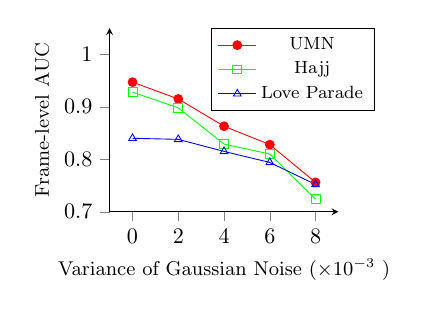
\begin{tikzpicture}[scale=0.8] 
\begin{axis}[
    width=0.43\textwidth,
    xlabel={\fontsize{9pt}{0}\selectfont Variance of Gaussian Noise ($\times 10^{-3}$ )}, 
    ylabel={\fontsize{9pt}{0}\selectfont Frame-level AUC}, 
    axis lines = left,
    xmin=-1,xmax=9,ymin=0.7,ymax=1.05,
    xtick={ 0,2,4,6,8},
    tick align=outside, 
    legend style={at={(0.8,1.0)},anchor=north} 
    ]

\addplot[mark=*,red] plot coordinates { 
    (0,0.947)
    (2,0.915)
    (4,0.863)
    (6,0.828)
    (8,0.756)
};
\addlegendentry{{\fontsize{8pt}{0}\selectfont UMN}}

\addplot[mark=square,green] plot coordinates {
    (0,0.928)
    (2,0.898)
    (4,0.829)
    (6,0.81)
    (8,0.724)
};
\addlegendentry{{\fontsize{8pt}{0}\selectfont Hajj}}

\addplot[mark=triangle,blue] plot coordinates { 
    (0,0.84)
    (2,0.838)
    (4,0.815)
    (6,0.794)
    (8,0.752)
};
\addlegendentry{{\fontsize{8pt}{0}\selectfont Love Parade}}
\end{axis}
\end{tikzpicture}
\caption{Frame-level AUC of our method when the variance of Gaussian noise changes.}
\label{fig: noise}
\end{figure}

\begin{table}[h]
\centering
\caption{Frame-level AUC of our method when the input datasets are downsampled.}
\label{downsample}
\begin{tabular}{l|c|c|c} 
\hline
\multirow{2}{*}{\diagbox{dataset}{resolution}} & \multirow{2}{*}{1x} & \multirow{2}{*}{0.75x} &  \multirow{2}{*}{0.5x} \\
                  &                     &                        &   \\
\hline
%UMN               &                     &                        &   \\
Hajj (high-res part) &    91.1\%     &   90.4\%      &   89.9\% \\
Love Parade          &    84.0\%     &   83.4\%      &   83.0\% \\
\hline
\end{tabular}
\end{table}

To simulate imperfect data situations in the real world, we conducted a downsampling of experimental data. The downsampling experiment was only conducted on Hajj and Love Parade because the resolution of UMN is already very low. This type of experiment can help us evaluate the performance of a system or model in the face of imperfect data, as well as its ability to adapt to abnormal situations. As we can see in Table~\ref{downsample}, the performances are not degraded too much (only by 1\% and 0.8\% in AUC).
Since our feature extraction method aggregates the neighboring pixels into one region, decreasing the resolution has little effect on our method.

\subsection{Evaluation on Risk Level Quantification}


\begin{figure}[t]
%\setlength{\abovecaptionskip}{+0.9cm}
%\setlength{\belowcaptionskip}{-0.5cm}
\centering
    \subfloat[Anomaly scores for different abnormal behaviors]{\includegraphics[width=3.4in]{figures/quantify-a.pdf}%
    \label{fig_a}}
    
    \subfloat[Existing metrics for different abnormal behaviors]{\includegraphics[width=3.4in]{figures/quantify-b.pdf}%
    \label{fig_b}}
    
    \subfloat[Our assessment for different abnormal behaviors]{\includegraphics[width=3.4in]{figures/quantify-c.pdf}%
    \label{fig_c}}
    \caption{
		Comparison of quantification results among original anomaly scores from MSMC-Net, existing metrics and our assessment method. 
}
\label{quantify}
\end{figure}

To evaluate the effectiveness of our assessment method for quantifying risk level of crowd anomalies, we conducted quantitative evaluation on different types of CABs on three datasets, including the escape in UMN, the counter flow in Hajj, and the crowd turbulence in Love Parade. We selected three well-known offline crowd risk metrics, namely particle entropy~\cite{gu2014abnormal}, collective consistency~\cite{zhou2013measuring} and crowd pressure~\cite{johansson2008crowd} for comparing with our method. Details on how
these compared metrics measure the crowd risk are described in Appendix. For the convenience of comparison, the min-max normalization was performed on the evaluation results obtained from each compared metric as well as our assessment method, linearly transforming the results into the value range of 0 to 1. Note that we classify these compared ones as offline metrics because the calculation of these metrics requires positional information of individuals in a crowd. In high-density crowd videos, it can take more than 60 ms per frame to track individual positions even using SOTA computer vision techniques, which make it impractical to use these compared metrics for online crowd risk monitoring. 

Fig.~\ref{quantify} shows the quantification of risk level of various CABs using our assessment method, compared to the original anomaly scores generated by our MSMC-Net and the existing metrics. Note that, for each dataset, we select one compared metric that has been verified in the same dataset or similar dataset, and show the corresponding quantification results in Fig.~\ref{quantify} (b). By comparing the results in Fig.~\ref{quantify} (a) and (c), it can be seen that our assessment method can effectively solve the problems of anomaly score as we mentioned in section~\ref{riskQuantification}: namely abrupt score increase at the start of CAB detection (see the dashed boxes a1 compared with c1, and a2 compared with c4 for examples) and score fluctuation when anomaly persists (see the dashed box a3 compared with c5 for example). By comparing the results in Fig.~\ref{quantify} (b) and (c), it can be also seen that our assessment of risk level is generally consistent with the changing trend of the normalized value of the existing offline metrics. Moreover, our method can produce smoother results (see the dashed box b1 compared with c2, b2 compared with c3, and b3 compared with c5 for examples), thanks to our double exponential smoothing mechanism. 


\subsection{Running Time}
Our framework is implemented with Pytorch. The experiments are performed on NVIDIA Tesla T4 GPUs with Intel(R) Xeon(R) 6230 2.10 GHz CPUs. 
The average running time of our trained model is approximately 75 ms, which contains crowd motion feature extraction (45 ms) and neural network computation (30 ms). The average running times of baseline methods, including AMC, FramePred, AMMC-Net, MNAD(recons), and MNAD(pred), are 81ms, 160ms, 55 ms, 34ms, and 61 ms, respectively, in our experiments. Overall, the average running time for executing our trained model to detect CABs in the testing videos is comparable to the baseline methods. 
The average running time of the assessment is about 75.3 ms, which includes generating abnormal scores (75 ms) and calculating risk levels (0.3 ms). This suggests that our risk assessment is efficient to be  executed for online crowd risk surveillance.

\section{Conclusion}
An unsupervised learning approach is introduced to perform crowd-level anomaly detection, which exploits the macroscopic patterns of crowd motion via multi-scale spatio-temporal motion consistency learning. Specifically, the spatial and temporal motion consistency is used to elicit the global and collective patterns in crowd motion. A multi-scale motion consistency network with a dual-attention mechanism is proposed to learn crowd motion features extracted at multi-scale and enable our model to estimate the proper scale of crowd behavior for detecting CABs. Furthermore, to quantify the risk level of detected CABs, we propose an assessment method that optimizes the anomaly score obtained from anomaly detection network to derive the risk level of CABs. The quantified risk level can help security personnel to comprehend the seriousness of detected CABs in real-time. Extensive evaluations based on real-world datasets demonstrate that our detection network outperforms the state-of-the-art VAD methods for detecting CABs and it can be applied to cross-dataset detection and robust to the noises. The experiment results on risk assessment show that our assessment method can generated quantified risk level that is consistent with the existing offline metrics and it has low running time to support online risk monitoring. Due to the complexity of crowd-level abnormal behaviors, our current method can only achieve frame-level detection. In future, we will work on improving the current framework to support pixel-level detection of CABs by fusing deep learning model with physics-informed crowd model.

\bibliographystyle{IEEEtran}
\bibliography{aaai23}


\clearpage
%\appendix
\thispagestyle{empty}
\section*{Supplementary material}\label{appendix}
% Section~\ref{appendix:curves}
\setcounter{figure}{0}
\setcounter{table}{0}
\setcounter{footnote}{0}
\noindent This supplementary material is organized as follows. First, we provide the algorithmic reconstruction procedure of our proposed MSMC-Net. Next, we describe the details of datasets used for model training and testing. Then, we provide the implementation details for our method and all the baseline methods. Lastly, we describe the compared metrics for the crowd risk quantification. 

\subsection{Summary of reconstruction procedure}
The reconstruction procedure of our MSMC-Net is shown in Algorithm~\ref{algo}.

\begin{algorithm}[]
\caption{Reconstruction procedure of our MSMC-Net}
\label{algo}
\textbf{Input}: MSMC graphs $ \{G^{s}\}_{s=1}^{S} $
%, trainable weight matrices of self-attention $W_{\mathrm{qry}}, W_{\mathrm{key}},W_{\mathrm{val}} $\\
%\textbf{Parameter}: Unified scale $w,h$\\
%\textbf{Output}: Fusion-based reconstructed edges $ \{\hat{\mathbf{E}}^{s}\}_{s=1}^{S} $, auxiliary reconstructed edges $ \{\hat{\mathbf{E}}_{Aux}^s\}_{s=1}^{S} $ and reshaped attention maps $ \{\tilde{\mathbf{A}}^{s}\}_{s=1}^{S} $.
\begin{algorithmic}[1] %[1] enables line numbers
\FOR{$s=1 \to S$}
\STATE $\mathbf{z}^s = {\mathrm{GCN}}^s\left( G^s\right)$ \# GCN encoding
\STATE $\tilde{\mathbf{z}}^{s} = {\mathrm{Unpooling}}^s\left( \mathbf{z}^s\right)$  \# reshape into a unified scale
\STATE $\{{\tilde{\alpha}}^{s}\}_{s=1}^{S}$ , $\{\tilde{\beta}^{s}\}_{s=1}^{S}$ = $\{\tilde{\mathbf{z}}^{s}\}_{s=1}^{S}$
\STATE Obtain multi-scale attention map $[a_{xy}^{s}]$ based on Eq.~\ref{form:5}
\STATE Obtain spatio-temporal attention map $[b_{xy}^{s}]$ based on Eq.~9-10
\ENDFOR

%\FOR{$x=1 \to w$}
%\FOR{$y=1 \to h$}
%\FOR{$s=1 \to S$}
%\STATE $\tilde{z}_{s} = {Unpooling}^s\left( z_s\right)$
%\ENDFOR
\STATE Obtain normalized multi-scale attention maps $\mathbb{A}$ based on Eq.~6-7
\STATE Obtain normalized spatio-temporal attention maps $\mathbb{B}$ based on Eq.~11-13
\STATE Obtain multi-scale fusion vector $\mathbf{z}_{\mathrm{msFus}}$ using Eq.~8
\STATE Obtain spatio-temporal fusion vector set $\{ \mathbf{z}_{\mathrm{stFus}}^{s} \}^{S}_{s=1} $ using Eq.~14
%\STATE $\mathbf{z}_{\mathrm{ms-stFus}}^{s}$ = $\mathbf{z}_{\mathrm{msFus}}$  $\oplus$ $\mathbf{z}_{\mathrm{stFus}}^{s}$
%\ENDFOR
%\ENDFOR

\FOR{$s=1 \to S$}
%\STATE Let $\mathbf{A}^{s}=\left [ \hat{a}_{xy}^{s}\right ], \mathbf{z}_{\mathrm{Fus}}=\left[ z_{\mathrm{Fus}}^{xy} \right] $
\STATE $\tilde{\mathbf{A}}^{s} = {\mathrm{Pooling}}^s\left( \mathbf{A}^s\right)$  \# reshape into original scales
\STATE $\tilde{\mathbf{B}}^{s} = {\mathrm{Pooling}}^s\left( \mathbf{B}^s\right)$  \# reshape into original scales
\STATE $\tilde{\mathbf{z}}_{\mathrm{msFus}}^s \oplus \tilde{\mathbf{z}}_{\mathrm{stFus}}^s = {\mathrm{Pooling}}^s\left( \mathbf{z}_{\mathrm{msFus}} \oplus \mathbf{z}_{\mathrm{stFus}}^{s}\right)$
%\STATE $\tilde{\mathbf{z}}_{\mathrm{stFus}}^s = {\mathrm{Pooling}}^s\left( \mathbf{z}_{\mathrm{stFus}}^{s}\right)$
\STATE $\hat{\mathbf{E}}_{\mathrm{Fus}}^{s}= {\mathrm{Decode}}\left(\tilde{\mathbf{z}}_{\mathrm{msFus}}^s \oplus \tilde{\mathbf{z}}_{\mathrm{stFus}}^s \oplus \tilde{\mathbf{z}}^s \right)$ \# part (b) reconstruction
\STATE $\hat{\mathbf{E}}_{\mathrm{Aux}}^{s}= {\mathrm{Decode}}\left(\mathbf{z}^{s}\right)$ \# part (c) reconstruction
\ENDFOR

\STATE \textbf{return} $ \{\hat{\mathbf{E}}_{\mathrm{Fus}}^{s}\}_{s=1}^{S} ,\{\hat{\mathbf{E}}_{\mathrm{Aux}}^s\}_{s=1}^{S} ,  \{\tilde{\mathbf{A}}^{s}\}_{s=1}^{S}  $ and $ \{\tilde{\mathbf{B}}^{s}\}_{s=1}^{S} $.
\end{algorithmic}
\end{algorithm}


%\vskip -0.1in
\subsection{Datasets}
\label{appendix:dataset}

\noindent \underline{\textbf{UMN}}\footnote{\url{http://mha.cs.umn.edu/Movies/Crowd-Activity-All.avi}}
is a video shot by CCTV at the University of Minnesota in 2006 (see Fig.~\ref{fig:4a}). The video contains three scenes. The video areas of the three scenes are 6 x 10 meters, 7 x 12 meters, and 10 x 9 meters, respectively. In the video, the walking pedestrians are considered normal, while the crowd escaping is abnormal. The original resolution of UMN is 320x240. As shown in Fig.~\ref{fig:4a}, a flashing text label appears whenever a frame is regarded as abnormal. To avoid the influence of these labels on the anomaly detection task, we trim off the text label area of all video frames and the trimmed video has a resolution of 320x213. The dataset is divided into non-overlapping training and testing parts. Our training set contains 4410 frames of normal behaviors and our testing set contains 3300 frames of both normal (1823 frames) and abnormal behaviors (1477 frames). For labeling the ground truth, we use the original label already provided in the dataset. 


\vskip 0.1in
\noindent \underline{\textbf{Hajj}}\footnote{\url{https://github.com/KAU-Smart-Crowd/Hajj_abnormal_behavior_detection}} comes from the surveillance video of Saudi Arabia's annual religious pilgrimage, including nine 45-second segments of dense crowds (see Fig.~\ref{fig:4b}). In these videos, abnormal behaviors include standing, sitting, sleeping, running, moving in the opposite or different direction of the crowd, and non-pedestrian movements, such as cars and wheelchairs. Among these abnormal behaviors, we select the crowd-level abnormal behavior, namely counter flow, for evaluation. The resolution of the videos is 720x576. The selected dataset is divided into non-overlapping training and testing parts. The training set contains 1500 frames without counter flow behavior and the testing set contains 1080 frames with both counter flow behavior (480 frames) and normal behavior (600 frames). For labeling the ground truth, we use the original label already provided in the dataset. 

\begin{figure}[t]
%\setlength{\abovecaptionskip}{+0.9cm}
%\setlength{\belowcaptionskip}{-0.5cm}
\centering
    \subfloat[Example screenshots in UMN dataset]{\includegraphics[width=3.4in]{figures/UMN.pdf}%
    \label{fig:4a}}
    
    \subfloat[Example screenshots in Hajj dataset]
    {\includegraphics[width=3.4in]{figures/Hajj.pdf}%
    \label{fig:4b}}
    
    \subfloat[Example screenshots in Love Parade dataset]
    {\includegraphics[width=3.4in]{figures/loveparade.pdf}%
    \label{fig:4c}}
    
    \subfloat[Example screenshots in MOT20 dataset]
    {\includegraphics[width=3.4in]{figures/MOT1.pdf}%
    \label{mot}}
    
    \caption{
Example screenshots in our benchmark datasets. The arrows are added to indicate the optical flow in the frame. It is worth noting that during anomalies in the UMN dataset, there is a flashing text label in the upper left corner (see screenshots of outdoor and indoor escape), which is trimmed in our experiments to avoid its influence.
}
\label{fig:data}
\end{figure}

\vskip 0.1in
\noindent\underline{\textbf{Love Parade}}\footnote{\url{https://loveparade2010doku.wordpress.com/2010/08/30/lopavent-\\ veroffentlicht-originalvideos-von-7-der-16-uberwachungskameras-der-loveparade-2010/}} contains surveillance videos from 7 monitoring locations within 3 hours before the love parade accident in 2012 (see Fig.~\ref{fig:4c}). The total length of all videos is over 23 hours and the crowd density in the videos reaches 11 people per square meter. The videos contain various CABs, including counter flow and crowd turbulence. We chose the videos from two of the cameras (4 and 13) in which counter flow and turbulence occurred and selected the video frames that contain the anomalies and are before and after the occurrence of anomalies. The selected dataset is divided into non-overlapping training and testing parts. The training set contains 2767 frames of normal behaviors and the testing set contains 1830 frames in total, in which 810 frames contain anomalies. For labeling the ground truth of the counter flow, frames are labeled based on whether the groups of pedestrians move in a counter-direction from the majority of the crowd. To label the ground truth of the crowd turbulence, we refer to the post-disaster analysis of the Love Parade disaster and label the crowd turbulence events according to the provided timeline~\cite{helbing2012crowd}.
The first testing video containing the crowd turbulence is clipped from 14:50 to 15:10 of the Camera\_13\_1620 video, and the turbulence starts at 15:00. The second testing video containing the crowd turbulence is clipped from 13:50 to 14:11 of Camera\_04\_1440 video, and the turbulence starts at 14:04.


\vskip 0.1in
\noindent 
\underline{\textbf{MOT20}}\footnote{\url{https://motchallenge.net/data/MOT20/}} contains 8 video sequences generated by monitoring of 5 different scenes, such as urban streets, indoor shopping malls, public transportation, etc., covering various challenging factors such as congestion, lighting changes, occlusion. These sequences contain different forms of movement, such as one-way flow, two-way flow, cross flow (see Fig.~\ref{mot}). The average number of people in each video frame is about 160. To verify the performance of our model on complex crowd movement behavior using the MOT20 dataset, we used these videos as training data for the model, and then evaluated the model using test sets from other datasets.

\thispagestyle{empty}
\subsection{Baseline Details}\label{appendix:baselines}

\noindent \underline{\textbf{FramePred}} \cite{liu2018future}: The algorithm adopts U-Net as a generator to predict the next frame. It adopts the constraints of appearance (intensity loss and gradient loss) to generate a high-quality image and motion (optical flow loss) and detects anomaly by predicting future frame. Experimental results show that the AUC of the algorithm on CUHK Avenue, UCSD ped1, UCSD ped2, and ShanghaiTech datasets are 0.851, 0.831, 0.954, and 0.728, respectively.

\vskip 0.03in
\noindent \underline{\textbf{AMC}} \cite{nguyen2019anomaly}: This algorithm is a classical anomaly detection work based on reconstruction. Anomaly detection is realized by combining Conv-AE and CNN of U-Net to reconstruct the frame, then comparing the difference between the reconstructed frame and the actual frame based on the patch scheme. Experimental results show that the AUC of the algorithm on CUHK Avenue and UCSD ped2 datasets are 0.869 and 0.962, respectively.

\vskip 0.03in
\noindent \underline{\textbf{MNAD (recons/pred)}} \cite{park2020learning}: It exploits multiple prototypes to consider the various behaviors of normal data and uses a memory module to record the prototypical patterns of the items in the memory. At the same time, two modes of anomaly detection, prediction, and reconstruction, are proposed. Based on the memory module, novel feature compactness and separability loss are proposed to train memory, which ensures the diversity and discrimination of memory items. Experiments show that the AUC values of the reconstruction-based scheme on UCSD ped2, CUHK Avenue, and ShanghaiTech datasets are 0.902, 0.828, and 0.698, respectively; The AUC of the prediction-based scheme is 0.970, 0.885 and 0.705, respectively.

\vskip 0.03in
\noindent \underline{\textbf{AMMC-Net}} \cite{cai2021appearance}: Inspired by the rules of recognizing abnormal frames from multi-modal signals, the appearance motion memory consistency network~(AMMC-Net) is proposed. The method fully uses the prior knowledge of appearance and motion signals and captures the corresponding relationship between them in the high-level feature space. Then, combined with multi-view features, a more fundamental and robust feature representation of conventional events is obtained, which can significantly increase the gap between abnormal and normal events. Experimental results show that the AUC of the algorithm on UCSD ped2, CUHK Avenue, and Shanghai tech datasets are 0.966, 0.866, and 0.737, respectively.


\begin{table}[t!]
    \centering
    \caption{Parameter settings}
    \resizebox{\linewidth}{!}{
    \begin{tabular}{ll}
        \hline
        Parameters                                         & Value (UMN, Hajj, LP) \\
        \hline
        
        self-attention dimension
        ($q,k,v$)                      & 32, 16, 32 \\
        graph embedding dimension($z$)  & 32, 16, 32 \\
        encoder network size  &     (32, 16), (16,8), (32, 16)\\
        learning rate                   & $ 3e^{-4} $, $ 1e^{-4} $, $ 3e^{-4} $ \\
        \hline
        $ \beta_{1} $ of Adam optimizer              & 0.9     \\
        $ \beta_{2} $ of Adam optimizer              & 0.999   \\
        \hline
        velocity direction categories ($D$)            & 8     \\
        length of sliding window ($m$)              & 20       \\
        sliding window step ($\tau$)                        & 1  \\
        multi-scale number ($S$)                  & 3  \\
        fusion loss weight ($ \lambda_\mathrm{Fus} $)      & 1 \\
        soft sharing loss weight ($ \lambda_\mathrm{Sof} $)    & 1 \\
        auxiliary loss weight  ($ \lambda_\mathrm{Aux} $)    & 1 \\
        moving average weight ($ \lambda_\mathrm{Mov} $)  & 0.2 \\
        random seed                                  & 42 \\
        %\hline
        %UMN learning rate                          & $ 1e^{-4} $ \\
        %Hajj learning rate                         & $ 3e^{-4} $ \\
        %Loveparade 
        \hline
    \end{tabular}
    }
    \label{hyper}
    \vskip -0.1in
\end{table}


\vskip -0.03in
\subsection{Implementation Details}\label{appendix:implementation}
All our experiments are conducted on a desktop PC with Intel(R) Xeon(R) CPU E5-1650 V4@3.60GHz and 32 GB RAM operated with a 64-bit Windows 10 system.


\noindent \underline{\textbf{MSMC-Net (Ours)}}
We use a grid search to set hyper-parameters on the test split, and our hyper-parameters tuned for each dataset can be found in Table~\ref{hyper}.
The decay rates ($ \beta_{1} $,$ \beta_{2} $) of the Adam optimizer~\cite{kingma2015adam} for network parameter tuning are set to 0.9 and 0.999, as suggested in the original paper. The number of velocity direction categories ($D$) is set to the typical number of 8, representing top, bottom, left, right, top left, bottom left, etc. Considering a moderate range of scales, our multi-scale framework is tested using the scale range of \{1x, 2x, 4x\} scales. To train all parts in a balanced way, we set an equal weight for the fusion loss, auxiliary loss, and soft sharing loss. Considering crowd behaviors tend to last for a period, the weight of the moving average ($ \lambda_\mathrm{Mov} $) is set to 0.2. The region size $w\times h$ of the baseline $1x$ scale for each dataset is determined by the average pixel size of pedestrians in the dataset's videos, as described in the Methodology section. The random seed is set to 42 when initializing the network's parameters using the random seed function provided in Python. Farneback optical flow\footnote{Farneb{\"a}ck, G. 2003. Two-frame motion estimation based on polynomial expansion. In SCIA, 363–370.} is obtained using OpenCV\footnote{\url{https://docs.opencv.org/2.4/modules/video/doc/motion_analysis_and_object_tracking.html?highlight=calcopticalflowfarneback}}. All codes are implemented in Python, and our MSMC-Net is trained using PyTorch\footnote{\url{https://pytorch.org/}}.

\vskip 0.03in
\noindent \underline{\textbf{FramePred}}~\cite{liu2018future} The code is obtained from the link\footnote{\url{https://github.com/StevenLiuWen/ano_pred_cvpr2018}} and a grid search is used to set the hyper-parameters on the same test split as used for tuning our method. The learning rates are set to ($2e^{-4}$, $2e^{-5}$), ($1e^{-4}$, $1e^{-5}$) and ($2e^{-4}$, $2e^{-5}$) on the three datasets respectively. As stated in the original paper, $\lambda_{int}$, $\lambda_{gd}$, $\lambda_{op}$ and $\lambda_{adv}$ vary from different datasets very slightly and they are set to 1.0, 1.0, 2.0 and 0.05, respectively. For a fair comparison, the sliding window size is set to 20, the same as in our method.

\vskip 0.03in
\noindent \underline{\textbf{AMC}}~\cite{nguyen2019anomaly}
The code is obtained from the link\footnote{\url{https://github.com/nguyetn89/Anomaly_detection_ICCV2019}} and a grid search is used to set the hyper-parameters on the same test split as used for tuning our method. The learning rates are set to ($1e^{-4}$, $1e^{-5}$), ($5e^{-5}$, $5e^{-6}$) and ($1e^{-4}$, $1e^{-5}$) on the three datasets, respectively.

\vskip 0.03in
\noindent \underline{\textbf{MNAD}}~\cite{park2020learning}
The code is obtained from the link\footnote{https://github.com/cvlab\-yonsei/MNAD} and a grid search is used to set the hyper-parameters on the same test split as used for tuning our method. For the reconstruction version of MNAD, the learning rates are set as $2e^{-5}$, $1e^{-5}$ and $2e^{-5}$, and $\lambda$ is set to 0.9, 0.7 and 0.6 for the three datasets, respectively. For the prediction version of MNAD, the learning rates are set as $2e^{-4}$, $1e^{-4}$ and $2e^{-4}$, and $\lambda$ is set to 0.9, 0.5 and 0.5 for the three datasets, respectively. As for the height $H$ and width $W$ of the query feature map, and the number of feature channels $C$ and memory items $M$ hardly vary among different datasets. They are set to 32, 32, 512 and 10 as the same as in the original paper. The sliding window size is set to 20, the same as in our method for a fair comparison.

\vskip 0.03in
\noindent \underline{\textbf{AMMC-Net}}~\cite{cai2021appearance}
The code is obtained from the link\footnote{https://github.com/NjuHaoZhang/AMMCNet\_AAAI2021} and a grid search is used to set the hyper-parameters on the same test split as used for tuning our method. The learning rates are set as $1e^{-3}$, $3e^{-4}$ and $1e^{-3}$ for the three datasets. According to the ablation study in the original paper, the memory item numbers $K$, memory size $N$ and memory dimension $D$ are set to 2, 64 and 256. For a fair comparison, the sliding window size is also set to 20, the same as in our method.


\vskip -0.03in
\thispagestyle{empty}
\subsection{Crowd Risk Metrics for Comparison}\label{appendix:riskmetrics}
\vskip -0.03in
\noindent \underline{\textbf{Particle entropy}}~\cite{gu2014abnormal} measures the degree of disorder in the distribution of crowds by treating them as particles based on their position distribution and velocity direction distribution. The calculation of particle entropy depends on the location distribution information of a given crowd. The calculation of particle entropy first divides the video frame into grids and then counts the distribution of crowd particles in both horizontal and vertical directions. The particle entropy in the horizontal and vertical directions is then calculated separately and then combined to obtain the particle entropy of an entire frame. The effectiveness of particle entropy was validated on the Crowd PETS09 dataset, and the effectiveness of particle entropy in evaluating the degree of disorder in crowds with abnormal escape situations has been validated on the UMN dataset.

\vskip 0.03in
\noindent \underline{\textbf{Collective consistency}}~\cite{zhou2013measuring} reflects the degree of consistency among individuals within a group by measuring the distribution of individual velocity directions. The calculation of collective consistency depends on the detailed trajectory information of crowd movement. Collective consistency first calculates the velocity correlation between each individual and the neighboring crowd based on \textit{K}-nearest neighbors and then calculates the crowd similarity along the path based on crowd trajectory information. Finally, average normalization is performed on all the paths in a frame to form collective consistency. Experimental analysis has been conducted to verify the effectiveness of collective consistency on crowd collective walking and lane formation.

\vskip 0.03in
\noindent \underline{\textbf{Crowd pressure}}~\cite{johansson2008crowd} measures the degree of crowding and pushing during crowd turbulence by calculating the variance of speed and combining it with crowd density. The calculation of crowd pressure depends on the location information of the crowd obtained by crowd tracking method, as well as the density and speed of the crowd measured based on tracking information. The calculation method for crowd pressure is the variance of velocity per unit area multiplied by crowd density. Experimental analysis has been conducted in Love Parade dataset demonstrating the ability of crowd pressure to quantify turbulence anomalies.


%\subsection{Evolving Anomaly Scores}\label{appendix:curves}
%\vskip -0.03in
%Figure~\ref{evo} shows how the anomaly score in our testing data is improved as the training of our MSMC-net is performed over epochs. As the training proceeds, it can be seen that our method can generate a higher score for abnormal behavior and a lower score for normal behavior. 


% \subsection{\yhy{(Optional) Detailed Explanation on Optical Flow and/or Consistency Representation}}


\end{document}


